%DIF 1c1
%DIF LATEXDIFF DIFFERENCE FILE
%DIF DEL pre-OJ-COMS draft
%DIF ADD OJ-COMS revision 2026-08-27
%DIF < \documentclass{ieeeaccess}
%DIF -------
\documentclass{IEEEoj} %DIF >
%DIF -------

\usepackage{cite}
\usepackage{amsmath,amssymb,amsfonts}
%DIF 5d5
%DIF < \usepackage{newtxtext}
%DIF -------
\usepackage{bm}
\usepackage{booktabs}
\usepackage{graphicx}
%DIF 9a8-9
\usepackage{orcidlink} %DIF >
\hypersetup{hidelinks} %DIF >
%DIF -------
\usepackage{textcomp}
\usepackage{url}

%DIF 12-13c13-14
%DIF < \vol{16}
%DIF < \year{2026}
%DIF -------
\AtBeginDocument{\definecolor{ojcolor}{cmyk}{0.93,0.59,0.15,0.02}} %DIF >
\def\OJlogo{\vspace{-4pt}\hskip-4pt\includegraphics[height=18pt]{ojcoms.png}} %DIF >
%DIF -------

\graphicspath{{../}{./}}

\newcommand{\rhoA}{\rho_{\mathrm{A}}}
\newcommand{\Peirp}{P_{\mathrm{EIRP}}}
\newcommand{\wbsar}{\mathrm{SAR}_{\mathrm{wb}}}
%DIF PREAMBLE EXTENSION ADDED BY LATEXDIFF
%DIF CFONT PREAMBLE %DIF PREAMBLE
\RequirePackage{color}\definecolor{RED}{rgb}{1,0,0}\definecolor{BLUE}{rgb}{0,0,1} %DIF PREAMBLE
\DeclareOldFontCommand{\sf}{\normalfont\sffamily}{\mathsf} %DIF PREAMBLE
\providecommand{\DIFadd}[1]{{\protect\color{blue} \sf #1}} %DIF PREAMBLE
\providecommand{\DIFdel}[1]{{\protect\color{red} \scriptsize #1}} %DIF PREAMBLE
%DIF SAFE PREAMBLE %DIF PREAMBLE
\providecommand{\DIFaddbegin}{} %DIF PREAMBLE
\providecommand{\DIFaddend}{} %DIF PREAMBLE
\providecommand{\DIFdelbegin}{} %DIF PREAMBLE
\providecommand{\DIFdelend}{} %DIF PREAMBLE
\providecommand{\DIFmodbegin}{} %DIF PREAMBLE
\providecommand{\DIFmodend}{} %DIF PREAMBLE
%DIF FLOATSAFE PREAMBLE %DIF PREAMBLE
\providecommand{\DIFaddFL}[1]{\DIFadd{#1}} %DIF PREAMBLE
\providecommand{\DIFdelFL}[1]{\DIFdel{#1}} %DIF PREAMBLE
\providecommand{\DIFaddbeginFL}{} %DIF PREAMBLE
\providecommand{\DIFaddendFL}{} %DIF PREAMBLE
\providecommand{\DIFdelbeginFL}{} %DIF PREAMBLE
\providecommand{\DIFdelendFL}{} %DIF PREAMBLE
%DIF LISTINGS PREAMBLE %DIF PREAMBLE
\RequirePackage{listings} %DIF PREAMBLE
\RequirePackage{color} %DIF PREAMBLE
\lstdefinelanguage{DIFcode}{ %DIF PREAMBLE
%DIF DIFCODE_CFONT %DIF PREAMBLE
  moredelim=[il][\color{red}\scriptsize]{\%DIF\ <\ }, %DIF PREAMBLE
  moredelim=[il][\color{blue}\sffamily]{\%DIF\ >\ } %DIF PREAMBLE
} %DIF PREAMBLE
\lstdefinestyle{DIFverbatimstyle}{ %DIF PREAMBLE
	language=DIFcode, %DIF PREAMBLE
	basicstyle=\ttfamily, %DIF PREAMBLE
	columns=fullflexible, %DIF PREAMBLE
	keepspaces=true %DIF PREAMBLE
} %DIF PREAMBLE
\lstnewenvironment{DIFverbatim}{\lstset{style=DIFverbatimstyle}}{} %DIF PREAMBLE
\lstnewenvironment{DIFverbatim*}{\lstset{style=DIFverbatimstyle,showspaces=true}}{} %DIF PREAMBLE
%DIF END PREAMBLE EXTENSION ADDED BY LATEXDIFF

\begin{document}

\DIFdelbegin %DIFDELCMD < \history{}
%DIFDELCMD < \doi{}
%DIFDELCMD < %%%
\DIFdelend \DIFaddbegin \receiveddate{XX Month, XXXX}
\reviseddate{XX Month, XXXX}
\accepteddate{XX Month, XXXX}
\publisheddate{XX Month, XXXX}
\currentdate{XX Month, XXXX}
\DIFaddend

\title{\DIFdelbegin \DIFdel{Image-Informed Urban Propagation and Route-Level Body }\DIFdelend \DIFaddbegin \DIFadd{Human-Centric 6G RF-EMF }\DIFaddend Exposure \DIFdelbegin \DIFdel{Across }\DIFdelend \DIFaddbegin \DIFadd{with AI-Assisted Digital Twins in }\DIFaddend Ten Cities\DIFdelbegin \DIFdel{at 15 GHz}\DIFdelend }

\author{\DIFdelbegin %DIFDELCMD < \uppercase{Robin Wydaeghe}\authorrefmark{1}%%%
\DIFdelend \DIFaddbegin \DIFadd{ROBIN WYDAEGHE~\orcidlink{0000-0002-1374-0118}}\IEEEauthorrefmark{1}\DIFaddend ,
\DIFdelbegin %DIFDELCMD < \uppercase{G\"unter Vermeeren}\authorrefmark{1}%%%
\DIFdelend \DIFaddbegin \DIFadd{G\"UNTER VERMEEREN~\orcidlink{0000-0002-5309-3808}}\IEEEauthorrefmark{1}\DIFaddend ,
\IEEEmembership{Member, IEEE},
\DIFdelbegin %DIFDELCMD < \uppercase{Emmeric Tanghe}\authorrefmark{1}%%%
\DIFdelend \DIFaddbegin \DIFadd{EMMERIC TANGHE~\orcidlink{0000-0003-0020-6466}}\IEEEauthorrefmark{1}\DIFaddend ,
\IEEEmembership{Member, IEEE},
and \DIFaddbegin \DIFadd{WOUT JOSEPH}\DIFaddend ~\DIFdelbegin %DIFDELCMD < \uppercase{Wout Joseph}\authorrefmark{1}%%%
\DIFdelend \DIFaddbegin \DIFadd{\orcidlink{0000-0002-8807-0673}}\IEEEauthorrefmark{1}\DIFaddend ,
\IEEEmembership{Senior Member, IEEE}}

\DIFdelbegin %DIFDELCMD < \address[1]{Department of Information Technology, Ghent University/IMEC,
%DIFDELCMD < 9052 Ghent, Belgium (e-mail: robin.wydaeghe@ugent.be)}
%DIFDELCMD < %%%
\DIFdelend \DIFaddbegin \affil{Department of Information Technology, Ghent University/IMEC,
9052 Ghent, Belgium}
\DIFaddend

\DIFdelbegin %DIFDELCMD < \markboth
%DIFDELCMD < {%%%
\DIFdel{Wydaeghe }%DIFDELCMD < \headeretal%%%
\DIFdel{: Image-Informed Urban Propagation and Route-Level Body Exposure Across Ten Cities}%DIFDELCMD < }
%DIFDELCMD < %%%
\DIFdelend \DIFaddbegin \corresp{CORRESPONDING AUTHOR: Robin Wydaeghe
(e-mail: robin.wydaeghe@ugent.be).}

\markboth{Human-Centric 6G RF-EMF Exposure with AI-Assisted Digital Twins in Ten Cities}
\DIFaddend {Wydaeghe \DIFdelbegin %DIFDELCMD < \headeretal%%%
\DIFdel{: Image-Informed Urban Propagation and Route-Level Body Exposure Across Ten Cities}\DIFdelend \DIFaddbegin \DIFadd{\textit{et al.}}\DIFaddend }

\DIFdelbegin %DIFDELCMD < \corresp{Corresponding author: Robin Wydaeghe
%DIFDELCMD < (e-mail: robin.wydaeghe@ugent.be).}
%DIFDELCMD <

%DIFDELCMD < %%%
\DIFdelend \begin{abstract}
\DIFdelbegin \DIFdel{Street-level radiofrequency exposure varies along a pedestrian route because
buildings change the direct and reflected fields, surface materials affect how
much power returns to the street, and }\DIFdelend \DIFaddbegin \DIFadd{Realistic urban radiofrequency electromagnetic-field (RF-EMF) assessment must
connect the field in a city to the power absorbed by }\DIFaddend the human body\DIFdelbegin \DIFdel{absorbs differently
depending on the direction of arrival. This
study projects }\DIFdelend \DIFaddbegin \DIFadd{. This
supports monitoring and epidemiological studies. The goal of
this study is to compute direction-aware whole-body specific absorption rate
(SAR) along pedestrian routes in ten cities. We combine }\DIFaddend 360-degree street
images\DIFdelbegin \DIFdel{onto a photogrammetric city mesh to identify surface materials along pedestrian routes }\DIFdelend \DIFaddbegin \DIFadd{, photogrammetric geometry, and AI-derived object and material labels in
a human-centric digital twin. Its agentic AI stage uses SAM~3 Agent for
material and vegetation labeling. The calculation places possible transmitters
along visible rooflines }\DIFaddend at 15~GHz\DIFdelbegin \DIFdel{. Transmitters are placed along the visible
roofline in proportion to its physical length. All results }\DIFdelend \DIFaddbegin \DIFadd{, traces direct and single-reflection paths,
and applies each arrival direction to an anatomical body model. Results }\DIFaddend are
normalized per unit product of \DIFdelbegin \DIFdel{areal }\DIFdelend source density and effective isotropic radiated
power\DIFdelbegin \DIFdel{(EIRP). The transport model treats direct
paths and one specular reflection exactly, estimates one diffuse reflection, and
stops. The arriving fields and their directions are then applied to a
56,024-element Duke body model. A geometric fixed-grid diagnostic covers ten urban locations in Europe, Latin America, and East Asia and finds a twofold
span in location-median whole-body SAR. Five of these locations are then studied
with image-derived materials along fixed pedestrian routes containing 73
}\DIFdelend \DIFaddbegin \DIFadd{. The ten routes contain 163 }\DIFaddend observation points, each \DIFdelbegin \DIFdel{calculated with 16 independent replicas of 200,000
primary rays and 4,096 angular output cells. In a controlled test scene, the
adjoint estimate and deterministic quadrature differ by at most 0.0616~dB for
the reflected term. An independent forward tracer gives a maximum difference
of 0.0344~dB. Route-median }\DIFdelend \DIFaddbegin \DIFadd{evaluated with 64
independent runs. The normalized route-median }\DIFaddend whole-body \DIFdelbegin \DIFdel{specific absorption rate differs by }\DIFdelend \DIFaddbegin \DIFadd{SAR ranges from
0.00902 to 0.129~m$^2$~kg$^{-1}$, }\DIFaddend a factor of \DIFdelbegin \DIFdel{13.34 across the five routes}\DIFdelend \DIFaddbegin \DIFadd{14.31}\DIFaddend . Direct paths \DIFdelbegin \DIFdel{carry the
largest share at all 67 }\DIFdelend \DIFaddbegin \DIFadd{give the
largest component at 156 of 157 }\DIFaddend points with line of sight\DIFaddbegin \DIFadd{. The single-reflection
specular component is largest at one point}\DIFaddend , while the \DIFdelbegin \DIFdel{diffuse reflection }\DIFdelend \DIFaddbegin \DIFadd{single-reflection diffuse component }\DIFaddend is
the only nonzero \DIFdelbegin \DIFdel{modeled contribution at six fully }\DIFdelend \DIFaddbegin \DIFadd{component at six }\DIFaddend shadowed points. \DIFdelbegin \DIFdel{The maximum change
from 12 to 16 replicas is 0.0436~dB, though lower-tail estimates in Mexico
City and Tokyo are less stable.
These results describe ten fixed-grid locations
and five }\DIFdelend \DIFaddbegin \DIFadd{Increasing the number of
runs from 48 to 64 changes the total at any point by at most 0.32\%. Validation
in a controlled scene gives maximum differences of 1.43\% against deterministic
quadrature and 0.80\% against an independent Sionna RT forward calculation.
The reported values apply to the }\DIFaddend selected routes under \DIFdelbegin \DIFdel{a fixed modeland }\DIFdelend \DIFaddbegin \DIFadd{the stated source model.
We }\DIFaddend do not estimate \DIFdelbegin \DIFdel{city-wide }\DIFdelend \DIFaddbegin \DIFadd{whole-city }\DIFaddend or deployed-network exposure.
\end{abstract}

\DIFdelbegin %DIFDELCMD < \begin{keywords}
%DIFDELCMD < %%%
\DIFdel{Body dosimetry, image-informed propagation}\DIFdelend \DIFaddbegin \begin{IEEEkeywords}
\DIFadd{AI-assisted digital twins, human-centric wireless systems}\DIFaddend , ray tracing,
\DIFdelbegin \DIFdel{street imagery, urban
propagation}\DIFdelend \DIFaddbegin \DIFadd{RF-EMF exposure}\DIFaddend , whole-body specific absorption rate.
\DIFdelbegin %DIFDELCMD < \end{keywords}
%DIFDELCMD < %%%
\DIFdelend \DIFaddbegin \end{IEEEkeywords}
\DIFaddend

\DIFdelbegin %DIFDELCMD < \titlepgskip%%%
\DIFdel{=-21pt
}\DIFdelend \maketitle

\section{Introduction}\label{sec:introduction}

\DIFdelbegin %DIFDELCMD < \IEEEPARstart{A}{s} %%%
\DIFdel{wireless networks expand into higher frequency bands,
the built environment plays a larger role in determining the radiofrequency field that reaches a pedestrian~\cite{itu2040}}\DIFdelend \DIFaddbegin \IEEEPARstart{R}{ealistic} \DIFadd{radiofrequency electromagnetic-field (RF-EMF)
exposure assessment must connect the field in a real environment to the power
absorbed by the human body. This link matters for street-level exposure
monitoring and for exposure estimates used in epidemiological research}\DIFaddend . Along
a city street, \DIFdelbegin \DIFdel{received
power can change over a few meters. A person walking past a row of buildings can move from a clear view of a rooftop transmitter into a shadow where
buildings }\DIFdelend \DIFaddbegin \DIFadd{buildings can }\DIFaddend block the direct field\DIFdelbegin \DIFdel{and only reflected power reaches the
street. The facade materials
then determine how much power returns to the street}\DIFdelend \DIFaddbegin \DIFadd{, and facade materials
change the reflected power}\DIFaddend ~\cite{itu2040,vitucci}. \DIFdelbegin \DIFdel{This variation also matters after the field
arrives: }\DIFdelend \DIFaddbegin \DIFadd{Human }\DIFaddend whole-body absorption
\DIFaddbegin \DIFadd{also }\DIFaddend depends on the \DIFdelbegin \DIFdel{direction of arrival and on how
the body is oriented, so a single power value at a single point does not
describe exposure }\DIFdelend \DIFaddbegin \DIFadd{arrival direction and body orientation~\cite{icnirp}.
Therefore, exposure assessment }\DIFaddend along a walking route \DIFdelbegin \DIFdel{. A route-level calculation must keep
the arrival }\DIFdelend \DIFaddbegin \DIFadd{must retain }\DIFaddend direction
until the field is applied to the body\DIFdelbegin \DIFdel{~\cite{icnirp}}\DIFdelend .

\DIFdelbegin \DIFdel{Ray tracing computes detailed propagation paths between transmitters and
receivers in a }\DIFdelend \DIFaddbegin \DIFadd{Prior exposure studies provide several parts of this link. Ray tracing gives
detailed paths in }\DIFaddend three-dimensional city \DIFdelbegin \DIFdel{model}\DIFdelend \DIFaddbegin \DIFadd{models}\DIFaddend ~\cite{sionna}. \DIFdelbegin \DIFdel{It has been used for
}\DIFdelend \DIFaddbegin \DIFadd{Ray tracing has supported
}\DIFaddend city-scale downlink exposure \DIFdelbegin \DIFdel{using published }\DIFdelend \DIFaddbegin \DIFadd{calculations with known }\DIFaddend base-station
locations~\cite{leeman} \DIFdelbegin \DIFdel{, and to compute propagation and }\DIFdelend \DIFaddbegin \DIFadd{and realistic 28~GHz }\DIFaddend body exposure along an outdoor
\DIFdelbegin \DIFdel{pedestrian }\DIFdelend path~\cite{wydaeghe2026}. Stochastic geometry \DIFdelbegin \DIFdel{models
describe exposure when individual transmitter
locationsare not
known~\cite{wiame}, while precomputed body coefficients separate the incident field from the absorptioncalculation}\DIFdelend \DIFaddbegin \DIFadd{represents unknown transmitter
locations~\cite{wiame}. SAR conversion factors connect incident fields to
absorption}\DIFaddend ~\cite{varsier}. \DIFdelbegin \DIFdel{Together, these studies cover deterministic urban propagation, spatial source models, and the
directional absorption step that converts the arriving field into absorbed power
on the body. Because they }\DIFdelend \DIFaddbegin \DIFadd{These studies }\DIFaddend use different source assumptions\DIFdelbegin \DIFdel{, their reported
exposure values are not directly comparable without a common source
normalization}\DIFdelend \DIFaddbegin \DIFadd{.
A common normalization is needed before their exposure values can be compared}\DIFaddend .

\DIFdelbegin \DIFdel{A photogrammetric city mesh gives accurate building geometry, but its
triangles
carry no material information. Street-level images can fill that gap}\DIFdelend \DIFaddbegin \DIFadd{Detailed photogrammetric geometry~\cite{google3d,blosm} does not identify its
surface materials. Street images can supply this information}\DIFaddend . The Mapillary
Vistas \DIFdelbegin \DIFdel{dataset provides a taxonomy for dense segmentation of }\DIFdelend \DIFaddbegin \DIFadd{data set provides object classes for }\DIFaddend street scenes~\cite{vistas}.
Kamari \emph{et al.} \DIFdelbegin \DIFdel{segment street-level images, project
the resulting material classes onto city geometry
, and use that geometry in
}\DIFdelend \DIFaddbegin \DIFadd{assign material classes from street images to city geometry
for }\DIFaddend millimeter-wave ray tracing~\cite{mmsv}. Xia \emph{et al.} \DIFdelbegin \DIFdel{use }\DIFdelend \DIFaddbegin \DIFadd{combine }\DIFaddend semantic
point-cloud \DIFdelbegin \DIFdel{classification and detailed scene reconstruction }\DIFdelend \DIFaddbegin \DIFadd{classes with detailed scenes }\DIFaddend for outdoor ray tracing at
2.8~GHz~\cite{xia2024}. \DIFdelbegin \DIFdel{Projecting image-derived materials onto
city geometry is therefore established. This study does not claim any of these
operations as new. It uses them to build a material map around fixed pedestrian
routes, keeping the default geometry-based material wherever the images give no
reliable label.
}\DIFdelend \DIFaddbegin \DIFadd{These studies show that multimodal scene data can
support radio propagation. They do not connect a common source model, retained
arrival directions, and human whole-body SAR across routes in several cities.
}\DIFaddend

\DIFdelbegin \DIFdel{This study combines these established parts in one fixed model.
Each }\DIFdelend \DIFaddbegin \DIFadd{To address this gap, we form an AI-assisted, human-centric digital twin from
}\DIFaddend 360-degree street \DIFdelbegin \DIFdel{image is aligned with the same photogrammetric city mesh used for ray
tracing, and the image labelsare projected onto that mesh to produce a material map. A common transmitter model distributes sources along the visible
roofline at every site. Rooflines are a natural choice: they are elevated, street-facing, and visible
from the route. Distributing transmitters in proportion to roofline length
avoids tying the result to any particular deployment. The ray tracer keeps
the direct, }\DIFdelend \DIFaddbegin \DIFadd{images and photogrammetric city geometry. Mask2Former assigns
object labels. SAM~3 Agent performs the agentic AI step by assigning material
and vegetation labels on visible surfaces. A common model
places possible transmitters along rooflines. The propagation calculation keeps
direct, single-reflection }\DIFaddend specular, and \DIFaddbegin \DIFadd{single-reflection }\DIFaddend diffuse components
separate, \DIFdelbegin \DIFdel{preserving }\DIFdelend \DIFaddbegin \DIFadd{with }\DIFaddend their arrival directions, until the \DIFdelbegin \DIFdel{field is applied to the body . The transport model
treats direct paths and one
specular reflection exactly, estimates one diffuse reflection , and stops there.
The route points are fixed case studies, not a population sample, and the
roofline transmitters are a model, not a measured deployment. To the best of the authors' knowledge, prior work has not combined aligned
360-degree street images, a common roofline transmitter model, and separate
transport components with their arrival directions in a single route-level body
exposure calculation.
}%DIFDELCMD <

%DIFDELCMD < %%%
\DIFdel{This study applies the method }\DIFdelend \DIFaddbegin \DIFadd{body calculation. The model
includes one reflection only.
}

\DIFadd{The goal of this study is to compute direction-aware human whole-body SAR along
pedestrian routes in ten cities }\DIFaddend at 15~GHz\DIFdelbegin \DIFdel{across ten urban locations. A geometric
fixed-grid diagnostic first characterizes all ten locations with geometry-based
}\DIFdelend \DIFaddbegin \DIFadd{. The routes contain 163 observation
points with image-derived surface }\DIFaddend materials and a \DIFdelbegin \DIFdel{fixed body orientation. Five of these locations are then studied
with image-derived materials along fixed pedestrian routes containing 73
observation points. Every result }\DIFdelend \DIFaddbegin \DIFadd{body model facing along each
walk. Every value }\DIFaddend is normalized per unit active-source areal density and per
unit effective isotropic radiated power (EIRP). The \DIFdelbegin \DIFdel{route-median
whole-body SAR values }\DIFdelend \DIFaddbegin \DIFadd{selected-route medians
}\DIFaddend differ by a factor of \DIFdelbegin \DIFdel{13.34 across the five routes. These
results describe fixed-grid locations and fixed routes under one source and
transport model. They }\DIFdelend \DIFaddbegin \DIFadd{14.31. We }\DIFaddend do not estimate population exposure\DIFdelbegin \DIFdel{or deployed-network
exposure }\DIFdelend \DIFaddbegin \DIFadd{,
whole-city exposure, or exposure from a deployed network}\DIFaddend .

This work makes the following three contributions.
\begin{enumerate}
  \item \DIFdelbegin \DIFdel{Aligned }\DIFdelend \DIFaddbegin \DIFadd{Multimodal fusion combines }\DIFaddend 360-degree street images \DIFdelbegin \DIFdel{supply traceable material labels to
  the same city mesh used for ray tracing}\DIFdelend \DIFaddbegin \DIFadd{and city geometry
  with Mask2Former object labels and SAM~3 Agent material labels in an
  AI-assisted digital twin}\DIFaddend . Surfaces without a reliable image label keep their
  geometry-based material.

  \item A \DIFdelbegin \DIFdel{roofline transmitter model and transport calculation keep
  direct ,
  specular, and diffuse }\DIFdelend \DIFaddbegin \DIFadd{normalized roofline source model and an adjoint ray tracer keep
  direct and once-reflected }\DIFaddend power separate, with arrival directions, until the
  field is applied to the body.

  \item \DIFdelbegin \DIFdel{An application across ten urban locations and five detailed pedestrian
  routes reports geometric screening, fixed-route exposure distributions, }\DIFdelend \DIFaddbegin \DIFadd{Results for ten routes quantify whole-body SAR, component shares,
  numerical convergence, surface-material sensitivity, and }\DIFaddend controlled
  \DIFdelbegin \DIFdel{first-diffuse validation,
  replica convergence, and the retained
  transport at the six observation points where buildings block all direct and
  specular paths}\DIFdelend \DIFaddbegin \DIFadd{single-reflection validation}\DIFaddend .
\end{enumerate}

\section{\DIFdelbegin \DIFdel{Method}\DIFdelend \DIFaddbegin \DIFadd{Methods}\DIFaddend }
\label{sec:method}

\subsection{Study \DIFdelbegin \DIFdel{Configuration}\DIFdelend \DIFaddbegin \DIFadd{configuration}\DIFaddend }
\label{sec:configuration}

Fig.~\ref{fig:configuration} shows the \DIFdelbegin \DIFdel{study }\DIFdelend configuration. A 360-degree street image
is aligned with a photogrammetric city mesh cropped to a 250~m radius around the
route. \DIFdelbegin \DIFdel{Object and material labels from the image are projected onto
}\DIFdelend \DIFaddbegin \DIFadd{Image labels are assigned to }\DIFaddend the visible mesh triangles without changing
their geometry. \DIFdelbegin \DIFdel{The roofline visible from the route gives the possible transmitter locations}\DIFdelend \DIFaddbegin \DIFadd{Possible transmitters lie along visible rooflines}\DIFaddend . Fixed
points \DIFdelbegin \DIFdel{along the
pedestrian route give }\DIFdelend \DIFaddbegin \DIFadd{set }\DIFaddend the observation positions, and the anatomical body model faces \DIFdelbegin \DIFdel{along }\DIFdelend the
direction of travel at each point.

\DIFdelbegin %DIFDELCMD < \begin{figure*}[!t]
%DIFDELCMD <   %%%
\DIFdelendFL \DIFaddbeginFL \begin{figure*}[!htb]
  \DIFaddendFL \centering
  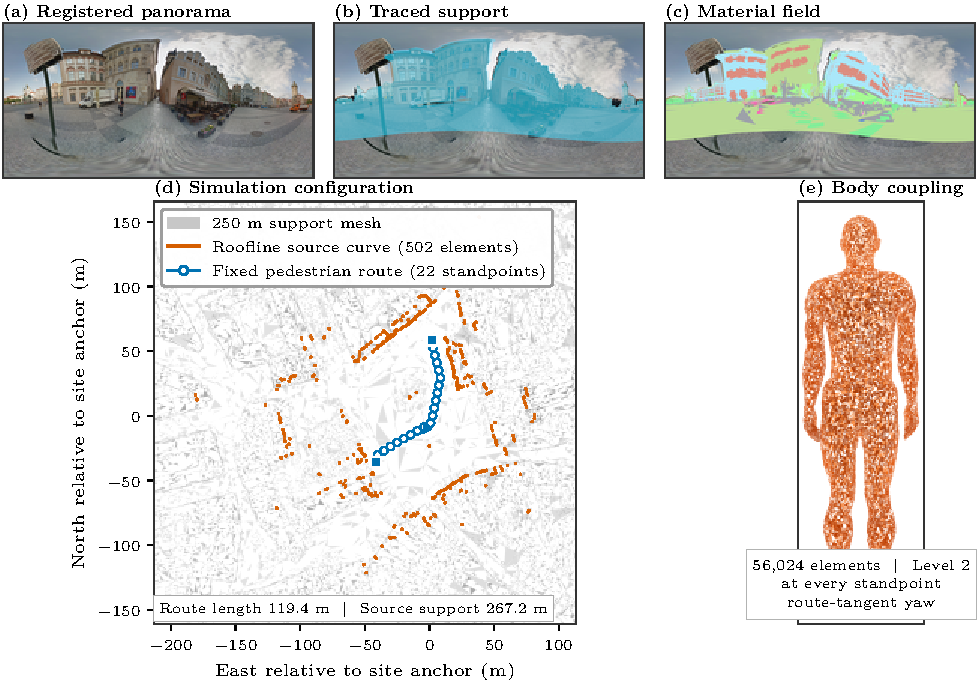
\includegraphics[width=\textwidth]{figures/configuration/configuration.pdf}
  \caption{\DIFdelbeginFL \DIFdelFL{Study configuration }\DIFdelendFL \DIFaddbeginFL \DIFaddFL{Configuration }\DIFaddendFL at Prague Old Town Square. (a) \DIFdelbeginFL \DIFdelFL{A }\DIFdelendFL \DIFaddbeginFL \DIFaddFL{Object and material labels from a }\DIFaddendFL 360-degree street image \DIFdelbeginFL \DIFdelFL{is segmented, projected onto the city mesh, and converted }\DIFdelendFL \DIFaddbeginFL \DIFaddFL{are assigned }\DIFaddendFL to the \DIFdelbeginFL \DIFdelFL{material map used for ray tracing}\DIFdelendFL \DIFaddbeginFL \DIFaddFL{city geometry}\DIFaddendFL . (b) \DIFdelbeginFL \DIFdelFL{The }\DIFdelendFL \DIFaddbeginFL \DIFaddFL{Plan view of the }\DIFaddendFL 22 observation points and \DIFdelbeginFL \DIFdelFL{the }\DIFdelendFL visible roofline\DIFdelbeginFL \DIFdelFL{on a plan view}\DIFdelendFL . (c) Close-up of the route. The arrow \DIFdelbeginFL \DIFdelFL{shows }\DIFdelendFL \DIFaddbeginFL \DIFaddFL{gives }\DIFaddendFL the body model's direction of travel.}
  \label{fig:configuration}
\end{figure*}

Table~\ref{tab:routes} lists the \DIFdelbegin \DIFdel{five selected routes}\DIFdelend \DIFaddbegin \DIFadd{study route in each of the ten cities}\DIFaddend . Each
route follows a connected street corridor covered by aligned 360-degree street
images. \DIFdelbegin \DIFdel{The
calculation places fixed observation points along that corridor, including
interpolated }\DIFdelend \DIFaddbegin \DIFadd{Fixed observation points include }\DIFaddend positions between image locations, so
the number of images and \DIFdelbegin \DIFdel{the number of observation }\DIFdelend points can differ. The \DIFdelbegin \DIFdel{73 route }\DIFdelend \DIFaddbegin \DIFadd{163 }\DIFaddend points are fixed \DIFdelbegin \DIFdel{observations, not a random sample of pedestrians or places. The body model
faces along the direction of travel, so a }\DIFdelend \DIFaddbegin \DIFadd{case-study
observations. Population and place sampling lie outside the study. A }\DIFaddend different route
would change both position and \DIFaddbegin \DIFadd{body }\DIFaddend orientation.

\begin{table}[!t]
  \caption{\DIFdelbeginFL \DIFdelFL{Five fixed routes }\DIFdelendFL \DIFaddbeginFL \DIFaddFL{Study route in each city, }\DIFaddendFL with observation-point counts, route spans, and \DIFdelbeginFL \DIFdelFL{computation }\DIFdelendFL \DIFaddbeginFL \DIFaddFL{ray calculation }\DIFaddendFL times}
  \label{tab:routes}
  \centering
  \begin{tabular}{lrrr}
    \toprule
    \DIFdelbeginFL \DIFdelFL{Site }\DIFdelendFL \DIFaddbeginFL \DIFaddFL{City }\DIFaddendFL & \DIFdelbeginFL \DIFdelFL{Route points }\DIFdelendFL \DIFaddbeginFL \DIFaddFL{Points }\DIFaddendFL & \DIFdelbeginFL \DIFdelFL{Route span }\DIFdelendFL \DIFaddbeginFL \DIFaddFL{Span }\DIFaddendFL (m) & \DIFdelbeginFL \DIFdelFL{Wall time }\DIFdelendFL \DIFaddbeginFL \DIFaddFL{Time }\DIFaddendFL (s) \\
    \midrule
    \DIFaddbeginFL \DIFaddFL{Brussels }& \DIFaddFL{14 }& \DIFaddFL{87.00 }& \DIFaddFL{32.16 }\\
    \DIFaddendFL Ghent & 10 & 49.04 & \DIFdelbeginFL \DIFdelFL{29.79 }\DIFdelendFL \DIFaddbeginFL \DIFaddFL{6.59 }\DIFaddendFL \\
    \DIFdelbeginFL \DIFdelFL{Prague }\DIFdelendFL \DIFaddbeginFL \DIFaddFL{Krakow }& \DIFaddFL{16 }& \DIFaddFL{116.10 }& \DIFaddFL{31.76 }\\
    \DIFaddFL{London }\DIFaddendFL & 22 & \DIFdelbeginFL \DIFdelFL{119.39 }\DIFdelendFL \DIFaddbeginFL \DIFaddFL{121.10 }\DIFaddendFL & \DIFdelbeginFL \DIFdelFL{69.02 }\DIFdelendFL \DIFaddbeginFL \DIFaddFL{73.77 }\DIFaddendFL \\
    Madrid & 14 & 73.47 & \DIFdelbeginFL \DIFdelFL{40.70 }\DIFdelendFL \DIFaddbeginFL \DIFaddFL{8.06 }\DIFaddendFL \\
    Mexico City & 11 & 60.79 & \DIFdelbeginFL \DIFdelFL{30.92 }\DIFdelendFL \DIFaddbeginFL \DIFaddFL{5.95 }\\
    \DIFaddFL{Milan }& \DIFaddFL{23 }& \DIFaddFL{128.43 }& \DIFaddFL{69.02 }\\
    \DIFaddFL{Prague }& \DIFaddFL{22 }& \DIFaddFL{119.39 }& \DIFaddFL{39.00 }\DIFaddendFL \\
    Tokyo Hachiko & 16 & 87.38 & \DIFdelbeginFL \DIFdelFL{50.11 }\DIFdelendFL \DIFaddbeginFL \DIFaddFL{10.02 }\\
    \DIFaddFL{Toulouse }& \DIFaddFL{15 }& \DIFaddFL{82.47 }& \DIFaddFL{37.87 }\DIFaddendFL \\
    \midrule
    Total & \DIFdelbeginFL \DIFdelFL{73 }\DIFdelendFL \DIFaddbeginFL \DIFaddFL{163 }\DIFaddendFL & \DIFdelbeginFL \DIFdelFL{390.07 }\DIFdelendFL \DIFaddbeginFL \DIFaddFL{925.17 }\DIFaddendFL & \DIFdelbeginFL \DIFdelFL{220.54 }\DIFdelendFL \DIFaddbeginFL \DIFaddFL{314.20 }\DIFaddendFL \\
    \bottomrule
  \end{tabular}
\end{table}

\DIFdelbegin \DIFdel{Two image-analysis models work }\DIFdelend \DIFaddbegin \subsection{\DIFadd{AI-assisted digital twin}}
\label{sec:digital-twin}

\DIFadd{Two image models are applied }\DIFaddend in sequence. Mask2Former assigns a Vistas object
class \DIFdelbegin \DIFdel{(}\DIFdelend \DIFaddbegin \DIFadd{such as }\DIFaddend building, road, \DIFdelbegin \DIFdel{vegetation, etc.) to every image
}\DIFdelend \DIFaddbegin \DIFadd{or vegetation to every }\DIFaddend pixel~\cite{mask2former,vistas}.
SAM~3 \DIFdelbegin \DIFdel{then tests }\DIFdelend \DIFaddbegin \DIFadd{Agent performs the agentic AI step by assigning }\DIFaddend material and vegetation
labels inside \DIFdelbegin \DIFdel{the }\DIFdelend compatible object regions~\cite{sam3}. \DIFdelbegin \DIFdel{Both sets of labels are
projected onto the visible city mesh using the known }\DIFdelend \DIFaddbegin \DIFadd{The }\DIFaddend camera position and
viewing direction \DIFdelbegin \DIFdel{. Where multiple images cover the same triangle, the }\DIFdelend \DIFaddbegin \DIFadd{locate these labels on visible triangles in the city geometry. When several images cover one
triangle, their accepted }\DIFaddend labels are combined\DIFdelbegin \DIFdel{into one material map, and every mapped triangle stays linked to its
source image. A mesh }\DIFdelend \DIFaddbegin \DIFadd{. A }\DIFaddend triangle changes material only
when \DIFdelbegin \DIFdel{the }\DIFdelend \DIFaddbegin \DIFadd{its }\DIFaddend object and material labels \DIFdelbegin \DIFdel{agree and pass the acceptance tests}\DIFdelend \DIFaddbegin \DIFadd{are compatible and meet the selection
criteria}\DIFaddend . All other triangles keep their \DIFdelbegin \DIFdel{default }\DIFdelend \DIFaddbegin \DIFadd{geometry-based }\DIFaddend material. The
\DIFaddbegin \DIFadd{supplementary material gives the }\DIFaddend prompts, alignment tests, rejected labels, and
\DIFdelbegin \DIFdel{mapping rulesare given in the supplementary material}\DIFdelend \DIFaddbegin \DIFadd{assignment rules}\DIFaddend .

Fig.~\ref{fig:flowchart} shows the \DIFdelbegin \DIFdel{computation and its input checks. A
hash-verified manifest lists every input file: aligned images, material map,
city mesh, route, roofline, body model, and transport settings. Only files whose
hashes match the manifest enter the five-site data set. The transport
calculation keeps direct, specular, and diffuse contributions separate until
the field is applied to the body. The five manifests contain 210 verified entries. Across the
resulting 1,168 directional body fields, the largest residual when the three
components are summed back to the stored total is
$1.735\times10^{-18}\,\mathrm{m}^{-2}$}\DIFdelend \DIFaddbegin \DIFadd{flowchart of the method}\DIFaddend .

\DIFdelbegin %DIFDELCMD < \begin{figure*}[!t]
%DIFDELCMD <   %%%
\DIFdelendFL \DIFaddbeginFL \begin{figure*}[!htb]
  \DIFaddendFL \centering
  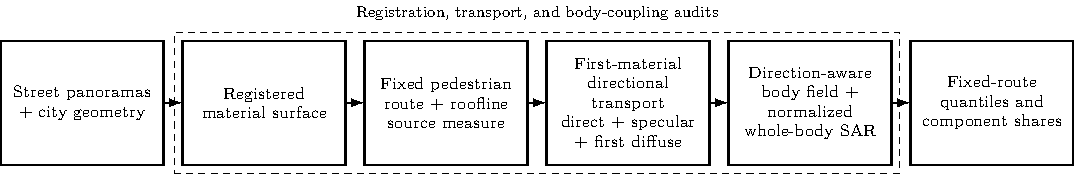
\includegraphics[width=\textwidth]{figures/flowchart/flowchart.pdf}
  \caption{Flowchart \DIFdelbeginFL \DIFdelFL{of the computation and input checks. Aligned 360-degree street images and the }\DIFdelendFL \DIFaddbeginFL \DIFaddFL{from multimodal }\DIFaddendFL city \DIFdelbeginFL \DIFdelFL{mesh give the material map}\DIFdelendFL \DIFaddbeginFL \DIFaddFL{data to whole-body specific absorption rate (SAR)}\DIFaddendFL . \DIFdelbeginFL \DIFdelFL{The fixed route and visible roofline give observation }\DIFdelendFL \DIFaddbeginFL \DIFaddFL{Mask2Former assigns object labels, }\DIFaddendFL and \DIFdelbeginFL \DIFdelFL{transmitter positions}\DIFdelendFL \DIFaddbeginFL \DIFaddFL{SAM~3 Agent assigns material labels}\DIFaddendFL . \DIFdelbeginFL \DIFdelFL{Transport retains direct}\DIFdelendFL \DIFaddbeginFL \DIFaddFL{These labels}\DIFaddendFL , \DIFdelbeginFL \DIFdelFL{first-order specular}\DIFdelendFL \DIFaddbeginFL \DIFaddFL{3-D city geometry}\DIFaddendFL , \DIFaddbeginFL \DIFaddFL{pedestrian locations }\DIFaddendFL and \DIFdelbeginFL \DIFdelFL{first-diffuse terms}\DIFdelendFL \DIFaddbeginFL \DIFaddFL{body orientations, and possible roofline transmitters form a human-centric digital twin}\DIFaddendFL . \DIFdelbeginFL \DIFdelFL{A hash-verified file list pins every input to the five-site result}\DIFdelendFL \DIFaddbeginFL \DIFaddFL{The propagation and body calculations then give whole-body SAR}\DIFaddendFL .}
  \label{fig:flowchart}
\end{figure*}

\subsection{Exposure \DIFdelbegin \DIFdel{Calculation}\DIFdelend \DIFaddbegin \DIFadd{calculation}\DIFaddend }
\label{sec:exposure-calc}

\DIFdelbegin \DIFdel{The calculation uses a fixed route, city mesh, material map, and roofline
transmitter model. }\DIFdelend Every route point uses 15~GHz and a \DIFaddbegin \DIFadd{circular scene }\DIFaddend crop with radius
$R_{\mathrm{crop}}=250$~m \DIFdelbegin \DIFdel{, which gives
$A_{\mathrm{crop}}=\pi R_{\mathrm{crop}}^2=196{,}349.54$}\DIFdelend \DIFaddbegin \DIFadd{and area
$A_{\mathrm{crop}}=196{,}349.54$}\DIFaddend ~m$^2$. The receiver position $\mathbf{x}$ is
the ray origin and body reference point. The body \DIFdelbegin \DIFdel{model faces along }\DIFdelend \DIFaddbegin \DIFadd{faces }\DIFaddend the local direction of
travel. Index $i$ denotes a roofline segment, $r_i(\mathbf{x})$ is its range to
the receiver, and $\mathbf{r}$ is a \DIFdelbegin \DIFdel{position }\DIFdelend \DIFaddbegin \DIFadd{point }\DIFaddend on the body surface.
\DIFdelbegin \DIFdel{These assumptions are fixed
across replicas and sites.
}\DIFdelend

\DIFdelbegin \DIFdel{The exact positions of future transmitters are unknown,
but elevated rooflines are plausible street-facing }\DIFdelend \DIFaddbegin \DIFadd{We consider a future distributed massive MIMO (DMaMIMO) architecture only to
define possible access-point locations~\cite{wydaeghe2026,ngo2017}. Therefore,
the model uses visible rooflines as possible transmitter }\DIFaddend locations. The \DIFdelbegin \DIFdel{model therefore distributes the
}\DIFdelend \DIFaddbegin \DIFadd{calculation does not model coordinated
transmission or beamforming. It distributes }\DIFaddend expected transmitters uniformly per
unit physical length of the roofline visible from the route. \DIFdelbegin \DIFdel{Let $\rho_A$ be the expected }\DIFdelend \DIFaddbegin \DIFadd{The }\DIFaddend active-site density \DIFdelbegin \DIFdel{and let
$A_{\mathrm{crop}}$ be the crop area}\DIFdelend \DIFaddbegin \DIFadd{$\rho_A$ gives an
expected count $N_{\mathrm{site}}=\rho_A A_{\mathrm{crop}}$}\DIFaddend . For a \DIFdelbegin \DIFdel{roofline }\DIFdelend segment with
endpoints $\mathbf{p}_i$ and $\mathbf{p}_{i+1}$, \DIFdelbegin \DIFdel{$\ell_i$ is its physical
three-dimensional length. The expected number of transmitters and the fraction assigned to segment $i$ are
}\begin{displaymath}
\DIFdel{N_{\mathrm{site}}=\rho_A A_{\mathrm{crop}},
\qquad
p_i=\frac{\ell_i}{\sum_j \ell_j},
\qquad
\ell_i=\left\lVert\mathbf{p}_{i+1}-\mathbf{p}_i\right\rVert_2 \, .
%DIFDELCMD < \label{eq:source-measure}%%%
}\end{displaymath}%DIFAUXCMD
\DIFdelend \DIFaddbegin \DIFadd{its source fraction is
}\begin{equation}
\DIFadd{p_i=\frac{\ell_i}{\sum_j \ell_j},\qquad
\ell_i=\lVert\mathbf{p}_{i+1}-\mathbf{p}_i\rVert_2 .
\label{eq:source-measure}
}\end{equation}\DIFaddend
\DIFdelbegin \DIFdel{Thus, $N_{\mathrm{site}}$ sets the number of transmitters and $p_i$ assigns a fraction of that number to segment $i$. Dividing by the total roofline length
ensures that splitting one segment into smaller numerical pieces does not add
transmitters. The baseline }\DIFdelend \DIFaddbegin \DIFadd{The denominator prevents a numerical split of one segment from adding source
power. The calculation }\DIFaddend uses three-dimensional length rather than horizontal
\DIFdelbegin \DIFdel{projected }\DIFdelend length.

An unobstructed reference separates \DIFdelbegin \DIFdel{the source density from the scene geometry. The reference sums the inverse-square contribution of every roofline segment}\DIFdelend \DIFaddbegin \DIFadd{source strength from scene geometry}\DIFaddend :
\begin{equation}
D_{\mathrm{ref}}(\mathbf{x})=
\sum_i\frac{p_i}{r_i(\mathbf{x})^2},
\qquad
S_{\mathrm{ref}}(\mathbf{x})=
\frac{A_{\mathrm{crop}}D_{\mathrm{ref}}(\mathbf{x})}{4\pi} \, .
\label{eq:reference-scale}
\end{equation}
\DIFdelbegin \DIFdel{No visibility test enters }\DIFdelend \DIFaddbegin \DIFadd{We apply no visibility test to }\DIFaddend $D_{\mathrm{ref}}$. All reported \DIFdelbegin \DIFdel{quantities }\DIFdelend \DIFaddbegin \DIFadd{values }\DIFaddend are
normalized per unit $\rho_A P_{\mathrm{EIRP}}$. Multiplication by
$\rho_A P_{\mathrm{EIRP}}$ \DIFdelbegin \DIFdel{recovers }\DIFdelend \DIFaddbegin \DIFadd{gives }\DIFaddend physical units, but only for a deployment
that follows the same roofline transmitter model. The calculation omits
transmitters and interactions outside the crop.

% claim: directional_component_representation
The propagation result at each observation point has direct, one-reflection
specular, and one-reflection diffuse parts. Let $\mathcal{D}$ contain \DIFdelbegin \DIFdel{the }\DIFdelend visible direct
paths \DIFdelbegin \DIFdel{, and let }\DIFdelend \DIFaddbegin \DIFadd{and }\DIFaddend $\mathcal{S}_1$ contain \DIFdelbegin \DIFdel{the }\DIFdelend accepted one-reflection specular
paths. Their normalized powers are
$\alpha_a=m_a^{(\mathrm{d})}/D_{\mathrm{ref}}$ and
$\beta_b=m_b^{(\mathrm{s})}/D_{\mathrm{ref}}$. The diffuse estimate uses
normalized angular-cell powers
$\widehat{\gamma}_q=\widehat{m}_q^{(\mathrm{f})}/D_{\mathrm{ref}}$ \DIFaddbegin \DIFadd{in
$Q=4096$ fixed angular cells}\DIFaddend . With $\delta_{\widehat{\mathbf{k}}}$ denoting a unit point
mass in \DIFdelbegin \DIFdel{physical }\DIFdelend arrival direction $\widehat{\mathbf{k}}$, the directional distribution is
\DIFdelbegin \begin{displaymath}
\DIFdel{\begin{aligned}
\mu_{\mathbf{x}}={}&
\sum_{a\in\mathcal{D}}\alpha_a\delta_{\widehat{\mathbf{k}}_a^{(\mathrm{d})}} \\
&+\sum_{b\in\mathcal{S}_1}\beta_b\delta_{\widehat{\mathbf{k}}_b^{(\mathrm{s})}} \\
&+\sum_{q=1}^{Q}\widehat{\gamma}_q\delta_{\widehat{\mathbf{k}}_q^{(\mathrm{f})}},
\qquad Q=4096 \, .
\end{aligned}
%DIFDELCMD < \label{eq:first-material-transfer}%%%
}\end{displaymath}%DIFAUXCMD
\DIFdelend \DIFaddbegin \begin{equation}
\DIFadd{\begin{aligned}
\mu_{\mathbf{x}}={}&
\sum_{a\in\mathcal{D}}\alpha_a\delta_{\widehat{\mathbf{k}}_a^{(\mathrm{d})}}
+\sum_{b\in\mathcal{S}_1}\beta_b\delta_{\widehat{\mathbf{k}}_b^{(\mathrm{s})}} \\
&+\sum_{q=1}^{Q}\widehat{\gamma}_q\delta_{\widehat{\mathbf{k}}_q^{(\mathrm{f})}} .
\end{aligned}
\label{eq:first-material-transfer}
}\end{equation}\DIFaddend
The first two sums \DIFdelbegin \DIFdel{retain the exact }\DIFdelend \DIFaddbegin \DIFadd{keep exact path }\DIFaddend directions and powers\DIFdelbegin \DIFdel{of the direct and
specular paths. They are not projected onto the angular grid}\DIFdelend . Only diffuse power
\DIFdelbegin \DIFdel{is accumulated in the $Q$ Fibonacci cells. Rays start at the
receiver and travel outward to the first blocking surface, as shown in
Fig.~\ref{fig:adjoint}. Next-event estimation then }\DIFdelend \DIFaddbegin \DIFadd{uses the angular cells. \emph{Adjoint ray tracing} launches rays from the
observation point and }\DIFaddend tests visibility from \DIFdelbegin \DIFdel{that surface }\DIFdelend \DIFaddbegin \DIFadd{each first surface hit }\DIFaddend to every
roofline \DIFdelbegin \DIFdel{segment}\DIFdelend \DIFaddbegin \DIFadd{source~\cite{behlouli2014,cocheril2007}. Fig.~\ref{fig:adjoint} shows
the difference from forward sampling. This source connection is a next-event
estimate}\DIFaddend ~\cite{veach}. The \DIFdelbegin \DIFdel{material model }\DIFdelend \DIFaddbegin \DIFadd{surface law }\DIFaddend combines unpolarized Fresnel power with
a Rayleigh roughness term. The \DIFdelbegin \DIFdel{remaining power enters }\DIFdelend \DIFaddbegin \DIFadd{surface law assigns the remaining reflected power to }\DIFaddend a
Lambertian diffuse \DIFdelbegin \DIFdel{term, and the }\DIFdelend \DIFaddbegin \DIFadd{component, and all }\DIFaddend components add incoherently. \DIFdelbegin \DIFdel{The }\DIFdelend \DIFaddbegin \DIFadd{Each }\DIFaddend sampled
path ends after \DIFdelbegin \DIFdel{this diffuse reflection, and the
calculation omits further specular reflections}\DIFdelend \DIFaddbegin \DIFadd{the diffuse reflection. Higher-order specular paths are also
omitted}\DIFaddend . Woody vegetation identified \DIFdelbegin \DIFdel{in
the material map }\DIFdelend \DIFaddbegin \DIFadd{by the images }\DIFaddend does not block rays because
the city \DIFdelbegin \DIFdel{mesh }\DIFdelend \DIFaddbegin \DIFadd{geometry }\DIFaddend has no canopy volume. The supplementary material gives the
full laws and \DIFdelbegin \DIFdel{parameter values}\DIFdelend \DIFaddbegin \DIFadd{parameters}\DIFaddend .

\DIFdelbegin %DIFDELCMD < \begin{figure*}[!t]
%DIFDELCMD <   %%%
\DIFdelendFL \DIFaddbeginFL \begin{figure*}[!htb]
  \DIFaddendFL \centering
  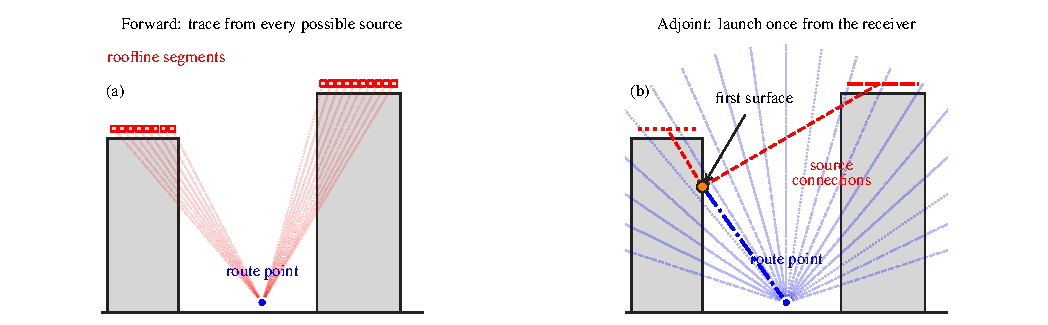
\includegraphics[width=\textwidth]{figures/adjoint/adjoint.pdf}
  \caption{Forward and adjoint sampling for the \DIFdelbeginFL \DIFdelFL{first-diffuse term}\DIFdelendFL \DIFaddbeginFL \DIFaddFL{single-reflection diffuse component}\DIFaddendFL . (a) \DIFdelbeginFL \DIFdelFL{A forward calculation }\DIFdelendFL \DIFaddbeginFL \DIFaddFL{Forward sampling }\DIFaddendFL launches rays from every roofline segment\DIFdelbeginFL \DIFdelFL{toward the observation point}\DIFdelendFL . (b) \DIFdelbeginFL \DIFdelFL{The adjoint calculation }\DIFdelendFL \DIFaddbeginFL \DIFaddFL{Adjoint sampling }\DIFaddendFL launches \DIFaddbeginFL \DIFaddFL{one set of }\DIFaddendFL rays \DIFdelbeginFL \DIFdelFL{once }\DIFdelendFL from the observation point \DIFdelbeginFL \DIFdelFL{. At }\DIFdelendFL \DIFaddbeginFL \DIFaddFL{and tests visible source connections at }\DIFaddendFL the first \DIFdelbeginFL \DIFdelFL{blocking }\DIFdelendFL surface \DIFdelbeginFL \DIFdelFL{, connections to every visible roofline segment are tested}\DIFdelendFL \DIFaddbeginFL \DIFaddFL{hit}\DIFaddendFL .}
  \label{fig:adjoint}
\end{figure*}

The \DIFdelbegin \DIFdel{arrival directions are carried through to the body }\DIFdelend \DIFaddbegin \DIFadd{calculation keeps each arrival direction until body coupling}\DIFaddend . For outward
\DIFdelbegin \DIFdel{body-surface }\DIFdelend \DIFaddbegin \DIFadd{surface }\DIFaddend normal $\widehat{\mathbf{n}}(\mathbf{r})$, \DIFdelbegin \DIFdel{define $g(\mathbf{r},\widehat{\mathbf{k}})=[\widehat{\mathbf{n}}(\mathbf{r})\cdot(-\widehat{\mathbf{k}})]_+$}\DIFdelend \DIFaddbegin \DIFadd{let
$g(\mathbf{r},\widehat{\mathbf{k}})=[\widehat{\mathbf{n}}(\mathbf{r})\cdot
(-\widehat{\mathbf{k}})]_+$}\DIFaddend . The normalized absorbed power density is
\DIFdelbegin \begin{displaymath}
\DIFdel{\begin{aligned}
\widetilde{S}_{\mathrm{ab}}(\mathbf{r},\mathbf{x})
&\equiv\frac{S_{\mathrm{ab}}(\mathbf{r},\mathbf{x})}{\rho_A P_{\mathrm{EIRP}}}
\\
&=T_0S_{\mathrm{ref}}(\mathbf{x})\Bigg[
\sum_{a\in\mathcal{D}}\alpha_a g(\mathbf{r},\widehat{\mathbf{k}}_a^{(\mathrm{d})}) \\
&\hspace{5.8em}+\sum_{b\in\mathcal{S}_1}\beta_b g(\mathbf{r},\widehat{\mathbf{k}}_b^{(\mathrm{s})}) \\
&\hspace{5.8em}+\sum_{q=1}^{Q}\widehat{\gamma}_q g(\mathbf{r},\widehat{\mathbf{k}}_q^{(\mathrm{f})})
\Bigg] \, .
\end{aligned}
%DIFDELCMD < \label{eq:body-coupling}%%%
}\end{displaymath}%DIFAUXCMD
\DIFdelend \DIFaddbegin \begin{equation}
\DIFadd{\widetilde{S}_{\mathrm{ab}}(\mathbf{r},\mathbf{x})
\equiv\frac{S_{\mathrm{ab}}(\mathbf{r},\mathbf{x})}{\rho_A P_{\mathrm{EIRP}}}
=T_0S_{\mathrm{ref}}(\mathbf{x})
\int_{\mathbb{S}^2}g(\mathbf{r},\widehat{\mathbf{k}})\,
\mathrm{d}\mu_{\mathbf{x}}(\widehat{\mathbf{k}}) .
\label{eq:body-coupling}
}\end{equation}\DIFaddend
\DIFaddbegin \DIFadd{The angular integral sums the direct, specular, and diffuse arrivals while
retaining their incoming directions.
}\DIFaddend Here, $T_0$ is the normal-incidence power-transmission coefficient from the
IT'IS tissue database at 15~GHz~\cite{itis}. It \DIFdelbegin \DIFdel{approximates the
absorption cross section for }\DIFdelend \DIFaddbegin \DIFadd{represents }\DIFaddend incoherent,
unpolarized illumination. The function $g$ \DIFdelbegin \DIFdel{sets the absorbed fraction to zero }\DIFdelend \DIFaddbegin \DIFadd{gives zero absorption }\DIFaddend where the
surface faces away from the incoming direction. \DIFdelbegin \DIFdel{The calculation applies this directional
absorption }\DIFdelend \DIFaddbegin \DIFadd{We apply this law }\DIFaddend to the
56,024-element Duke anatomical mesh~\cite{christ2010}. \DIFdelbegin \DIFdel{Because all quantities are normalized by $\rho_A P_{\mathrm{EIRP}}$,
$\widetilde{S}_{\mathrm{ab}}$ is dimensionless. For the }\DIFdelend \DIFaddbegin \DIFadd{With }\DIFaddend triangle area
$A_{\mathbf{r}}$ \DIFdelbegin \DIFdel{at position $\mathbf{r}$ }\DIFdelend and body mass $m_{\mathrm{body}}$, the normalized \DIFdelbegin \DIFdel{integrated quantities are
}\begin{displaymath}
\DIFdel{\begin{aligned}
\widetilde{P}_{\mathrm{abs}}(\mathbf{x})
&\equiv\frac{P_{\mathrm{abs}}(\mathbf{x})}{\rho_A P_{\mathrm{EIRP}}}
\\
&=\sum_{\mathbf{r}}A_{\mathbf{r}}\widetilde{S}_{\mathrm{ab}}(\mathbf{r},\mathbf{x}), \\
\widetilde{\mathrm{SAR}}_{\mathrm{wb}}(\mathbf{x})
&\equiv\frac{\mathrm{SAR}_{\mathrm{wb}}(\mathbf{x})}{\rho_A P_{\mathrm{EIRP}}}
\\
&=\frac{\widetilde{P}_{\mathrm{abs}}(\mathbf{x})}{m_{\mathrm{body}}} \, .
\end{aligned}
%DIFDELCMD < \label{eq:body-endpoints}%%%
}\end{displaymath}%DIFAUXCMD
\DIFdelend \DIFaddbegin \DIFadd{endpoints are
}\begin{equation}
\DIFadd{\begin{aligned}
\widetilde{P}_{\mathrm{abs}}(\mathbf{x})
&=\sum_{\mathbf{r}}A_{\mathbf{r}}\widetilde{S}_{\mathrm{ab}}(\mathbf{r},\mathbf{x}), \\
\widetilde{\mathrm{SAR}}_{\mathrm{wb}}(\mathbf{x})
&=\frac{\widetilde{P}_{\mathrm{abs}}(\mathbf{x})}{m_{\mathrm{body}}} .
\end{aligned}
\label{eq:body-endpoints}
}\end{equation}\DIFaddend
$\widetilde{P}_{\mathrm{abs}}$ has units m$^2$, and
$\widetilde{\mathrm{SAR}}_{\mathrm{wb}}$ has units m$^2$~kg$^{-1}$ \DIFaddbegin \DIFadd{per unit
$\rho_A P_{\mathrm{EIRP}}$}\DIFaddend .

\DIFdelbegin \DIFdel{Each replica }\DIFdelend \DIFaddbegin \subsection{\DIFadd{Numerical settings and route statistics}}
\label{sec:numerical-settings}

\DIFadd{For each independent run, the calculation }\DIFaddend launches 200,000 \DIFdelbegin \DIFdel{independent and identically distributed }\DIFdelend primary rays per
\DIFdelbegin \DIFdel{route point and accumulates first-diffuse }\DIFdelend \DIFaddbegin \DIFadd{observation point and collects single-reflection diffuse }\DIFaddend power in 4,096 fixed
\DIFdelbegin \DIFdel{Fibonacci output cells. Exact direct }\DIFdelend \DIFaddbegin \DIFadd{angular cells. Direct }\DIFaddend and specular paths \DIFdelbegin \DIFdel{bypass this grid. The output cells do }\DIFdelend \DIFaddbegin \DIFadd{are not binned on this grid, which does
}\DIFaddend not control the launch directions. The calculations use \DIFdelbegin \DIFdel{16 replicas }\DIFdelend \DIFaddbegin \DIFadd{64 runs }\DIFaddend with seeds 7
through \DIFdelbegin \DIFdel{22 and retain }\DIFdelend \DIFaddbegin \DIFadd{70 and keep }\DIFaddend cumulative results after 4, 8, 12, \DIFdelbegin \DIFdel{and }\DIFdelend 16\DIFdelbegin \DIFdel{replicas}\DIFdelend \DIFaddbegin \DIFadd{, 32, 48, and 64 runs}\DIFaddend .
Only the \DIFdelbegin \DIFdel{first-diffuse }\DIFdelend \DIFaddbegin \DIFadd{diffuse }\DIFaddend estimate varies between \DIFdelbegin \DIFdel{replicas. Scalar quantities }\DIFdelend \DIFaddbegin \DIFadd{runs. Scalar values }\DIFaddend and body fields
are averaged \DIFdelbegin \DIFdel{across replicas
}\DIFdelend before route statistics are computed. \DIFaddbegin \DIFadd{The ten routes give 10,432
directional body fields from 2.086 billion primary rays. }\DIFaddend Route quantiles use
linear interpolation over equally weighted \DIFdelbegin \DIFdel{route }\DIFdelend points, and \DIFdelbegin \DIFdel{the plotted empirical distributions use
positions }\DIFdelend \DIFaddbegin \DIFadd{empirical distribution
positions are }\DIFaddend $(\operatorname{rank}-0.5)/n$. \DIFdelbegin \DIFdel{Multipath surplus }\DIFdelend \DIFaddbegin \DIFadd{Excess above direct-path power }\DIFaddend is
computed only where direct \DIFdelbegin \DIFdel{transfer }\DIFdelend \DIFaddbegin \DIFadd{power }\DIFaddend is positive. \DIFdelbegin \DIFdel{A route point }\DIFdelend \DIFaddbegin \DIFadd{Points }\DIFaddend with zero direct \DIFdelbegin \DIFdel{transfer
remains in the whole-body }\DIFdelend \DIFaddbegin \DIFadd{power
remain in the }\DIFaddend SAR distribution but \DIFdelbegin \DIFdel{has no finite surplus value. }%DIFDELCMD <

%DIFDELCMD < %%%
\section{\DIFdel{Results}}
%DIFAUXCMD
\addtocounter{section}{-1}%DIFAUXCMD
%DIFDELCMD < \label{sec:results}
%DIFDELCMD <

%DIFDELCMD < %%%
%DIF <  claim: current_campaign_contract
\DIFdel{Table~\ref{tab:routes} defines the five fixed routes and their 73 observation
points. Every site uses 15~GHz and a photogrammetric city mesh cropped to a
250~m radius. The Duke body model has 56,024 surface elements and a mass of
72.4~kg, and faces along the direction of travel. Each point has 16 independent
replicas with seeds 7 through 22. Each replica uses 200,000 primary rays and
4,096 fixed Fibonacci output cells for the first-diffuse term. The resulting 1,168 body fields contain 233.6 million primary rays.
Calculation time for a prepared site ranges from 29.79 to 69.02~s on one }\DIFdelend \DIFaddbegin \DIFadd{have no finite excess value. Ray calculation
takes 5.95 to 73.77~s per city on one NVIDIA }\DIFaddend A6000 GPU. These times exclude
image acquisition, alignment, \DIFdelbegin \DIFdel{depth estimation, and material mapping because the full
preparation time was }\DIFdelend \DIFaddbegin \DIFadd{and surface-label assignment because their full
times were }\DIFaddend not recorded.

\DIFaddbegin \section{\DIFadd{Results}}
\label{sec:results}

\DIFaddend \subsection{Validation}
\label{sec:validation}

%DIF <  claim: raw_component_closure
\DIFdelbegin \DIFdel{The calculation manifests list 42 files per site, and all 210 file hashes pass
verification. The direct, exact order-1 specular, and first-diffuse fields sum
to the stored total with a maximum absolute residual of
$1.735\times10^{-18}$~m$^{-2}$ across all 1,168 fields. The GPU body-coupling
result also agrees with the double-precision CPU reference to a maximum relative
difference of $6.64\times10^{-16}$ in the verified benchmark. These checks
confirm the input files, addition of components, and agreement between CPU and
GPU calculations. They do not externally validate the complete city model.
}%DIFDELCMD <

%DIFDELCMD < %%%
\DIFdelend % claim: controlled_depth1_validation
\DIFdelbegin \DIFdel{The direct and specular paths are computed from exact geometry, but the
first-diffuse estimatedepends on random ray sampling. The controlled comparison
in }\DIFdelend \DIFaddbegin \DIFadd{Validation against deterministic quadrature and Sionna RT tests the
single-reflection diffuse estimate. }\DIFaddend Fig.~\ref{fig:controlled-validation} \DIFdelbegin \DIFdel{tests this stochastic component before
the city results. The }\DIFdelend \DIFaddbegin \DIFadd{shows
the comparison in an }\DIFaddend open-square scene \DIFdelbegin \DIFdel{has }\DIFdelend \DIFaddbegin \DIFadd{with }\DIFaddend 27 sources, 6 receivers, 8
triangles, and one diffuse reflection. \DIFdelbegin \DIFdel{It }\DIFdelend \DIFaddbegin \DIFadd{The scene }\DIFaddend has no specular reflection,
refraction, or diffraction. Deterministic surface quadrature uses 2,097,152
samples. The adjoint \DIFdelbegin \DIFdel{estimate }\DIFdelend \DIFaddbegin \DIFadd{calculation }\DIFaddend uses 50,000 primary rays for each of four
seeds. \DIFdelbegin \DIFdel{An }\DIFdelend \DIFaddbegin \DIFadd{The }\DIFaddend independent Sionna RT forward calculation uses 50,000 samples per
source for each of three seeds. The maximum \DIFdelbegin \DIFdel{difference
between the adjoint estimate and quadrature is
0.0616~dB }\DIFdelend \DIFaddbegin \DIFadd{adjoint-to-quadrature difference is
1.43\% }\DIFaddend for the reflected \DIFdelbegin \DIFdel{term}\DIFdelend \DIFaddbegin \DIFadd{component}\DIFaddend . A separate \DIFdelbegin \DIFdel{test of total transport }\DIFdelend \DIFaddbegin \DIFadd{comparison of total received
power }\DIFaddend gives a maximum adjoint-to-Sionna difference of \DIFdelbegin \DIFdel{0.0344~dB. Fig. ~\ref{fig:controlled-validation} plots the one-reflection
transfer and its error relative to quadrature, not the total-transport test. The
comparison checks first-diffuse }\DIFdelend \DIFaddbegin \DIFadd{0.80\%. The figure shows
the reflected component and its signed percentage difference from quadrature. This test
covers diffuse }\DIFaddend normalization, visibility, inverse-square loss, and cosine terms
in \DIFdelbegin \DIFdel{this }\DIFdelend \DIFaddbegin \DIFadd{a }\DIFaddend one-reflection scene. It does not \DIFdelbegin \DIFdel{cover }\DIFdelend \DIFaddbegin \DIFadd{validate }\DIFaddend the image-derived \DIFdelbegin \DIFdel{material map, exact specular transport}\DIFdelend \DIFaddbegin \DIFadd{surface
materials, the specular component}\DIFaddend , or their combination in a city.

\DIFdelbegin %DIFDELCMD < \begin{figure*}[!t]
%DIFDELCMD < %%%
\DIFdelendFL \DIFaddbeginFL \begin{figure*}[!htb]
\DIFaddendFL \centering
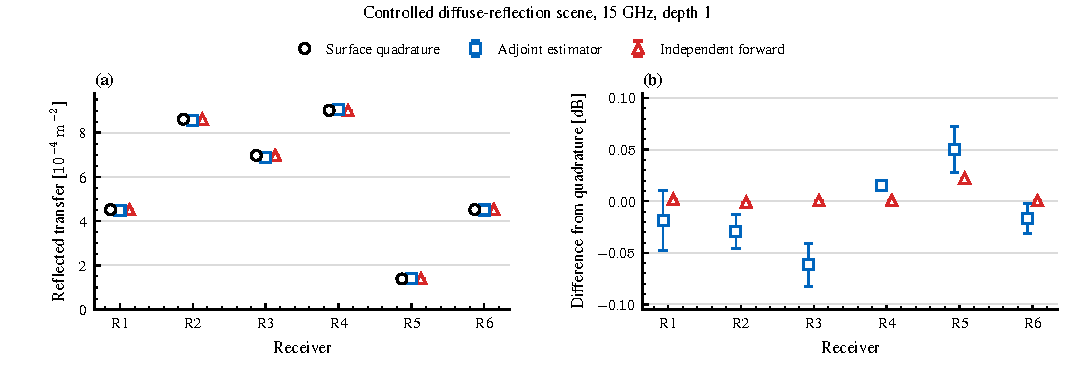
\includegraphics[width=\textwidth]{figures/validation/validation.pdf}
\caption{Controlled validation of the \DIFdelbeginFL \DIFdelFL{first-diffuse transfer}\DIFdelendFL \DIFaddbeginFL \DIFaddFL{single-reflection diffuse component}\DIFaddendFL . (a) Deterministic surface quadrature, the adjoint estimate, and the independent Sionna RT forward calculation at six receivers. (b) Signed \DIFdelbeginFL \DIFdelFL{error relative to }\DIFdelendFL \DIFaddbeginFL \DIFaddFL{percentage difference from }\DIFaddendFL quadrature. Error bars give the standard error across four adjoint seeds and three Sionna seeds.}
\label{fig:controlled-validation}
\end{figure*}

\subsection{Route \DIFdelbegin \DIFdel{Exposure}\DIFdelend \DIFaddbegin \DIFadd{exposure}\DIFaddend }
\label{sec:route-exposure}

%DIF <  claim: route_median_contrast_factor
%DIF >  claim: ten_route_median_contrast_factor
Fig.~\ref{fig:route-distributions} shows the fixed-route empirical distributions.
Table~\ref{tab:route-results} gives the \DIFdelbegin \DIFdel{central
summaries and finite multipath surplus}\DIFdelend \DIFaddbegin \DIFadd{route quantiles and excess above
direct-path power}\DIFaddend . Normalized whole-body SAR is reported in m$^2$~kg$^{-1}$ per
unit $\rho_A P_{\mathrm{EIRP}}$. A physical \DIFdelbegin \DIFdel{whole-body SAR value therefore }\DIFdelend \DIFaddbegin \DIFadd{value }\DIFaddend requires multiplication by \DIFdelbegin \DIFdel{the
}\DIFdelend \DIFaddbegin \DIFadd{a
}\DIFaddend deployment's areal source density and EIRP. The figure includes all \DIFdelbegin \DIFdel{73 }\DIFdelend \DIFaddbegin \DIFadd{163
}\DIFaddend observation points and marks the six with zero direct and zero
\DIFdelbegin \DIFdel{order-1 specular transfer}\DIFdelend \DIFaddbegin \DIFadd{single-reflection specular power}\DIFaddend . The largest \DIFdelbegin \DIFdel{route median is 13.34 }\DIFdelend \DIFaddbegin \DIFadd{selected-route median (Mexico City,
0.1291~m$^2$~kg$^{-1}$) is 14.31 }\DIFaddend times the smallest \DIFaddbegin \DIFadd{(Milan,
0.009016~m$^2$~kg$^{-1}$)}\DIFaddend . Mexico City and Tokyo Hachiko have the widest spread
along a route and the lowest tails.

\DIFdelbegin %DIFDELCMD < \begin{figure}[!t]
%DIFDELCMD < %%%
\DIFdelendFL \DIFaddbeginFL \begin{figure*}[!htb]
\DIFaddendFL \centering
\DIFdelbeginFL %DIFDELCMD < 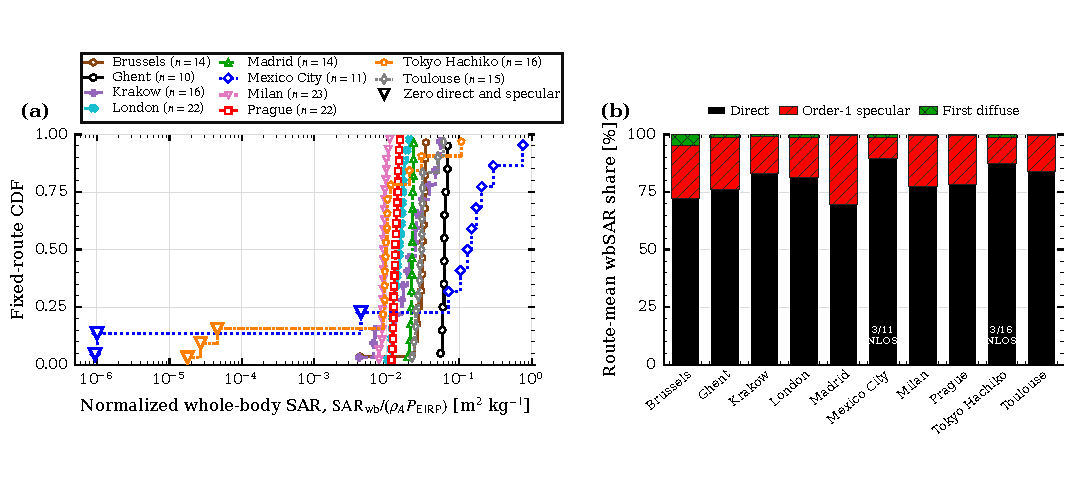
\includegraphics[width=\columnwidth]{figures/route_results/route_results.pdf}
%DIFDELCMD < %%%
\DIFdelendFL \DIFaddbeginFL 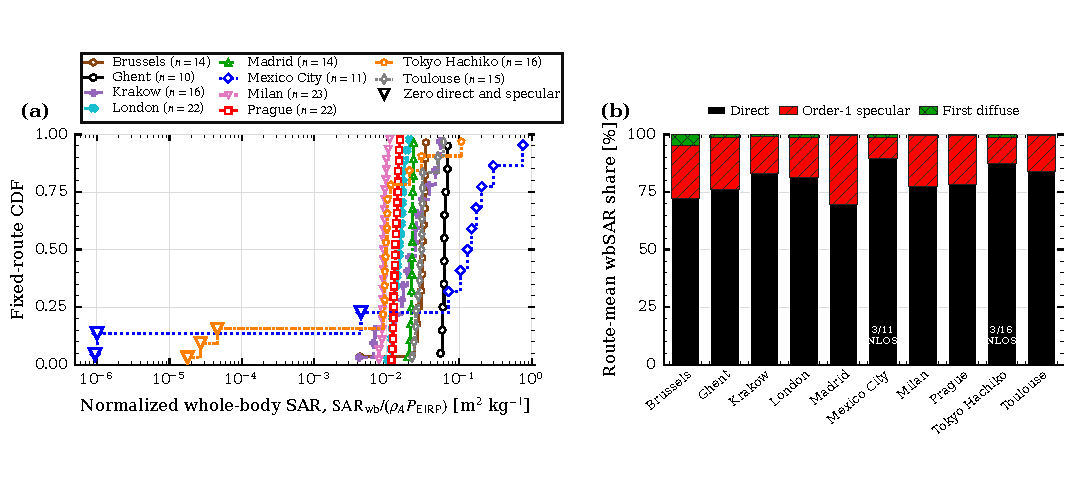
\includegraphics[width=\textwidth,height=0.76\textheight,keepaspectratio]{figures/route_results/route_results.pdf}
\DIFaddendFL \caption{Normalized whole-body SAR on the \DIFdelbeginFL \DIFdelFL{five }\DIFdelendFL \DIFaddbeginFL \DIFaddFL{ten }\DIFaddendFL fixed routes. \DIFaddbeginFL \DIFaddFL{(a)~}\DIFaddendFL Empirical CDFs include all \DIFdelbeginFL \DIFdelFL{73 route }\DIFdelendFL \DIFaddbeginFL \DIFaddFL{163 observation }\DIFaddendFL points. Hollow triangles mark the six points with zero direct and zero \DIFdelbeginFL \DIFdelFL{order-1 }\DIFdelendFL \DIFaddbeginFL \DIFaddFL{single-reflection }\DIFaddendFL specular \DIFdelbeginFL \DIFdelFL{transfer}\DIFdelendFL \DIFaddbeginFL \DIFaddFL{power. (b)~Route-mean component shares}\DIFaddendFL . The routes are \DIFdelbeginFL \DIFdelFL{fixed }\DIFdelendFL case studies \DIFdelbeginFL \DIFdelFL{, not }\DIFdelendFL \DIFaddbeginFL \DIFaddFL{and support no }\DIFaddendFL city or population \DIFdelbeginFL \DIFdelFL{samples}\DIFdelendFL \DIFaddbeginFL \DIFaddFL{inference}\DIFaddendFL .}
\label{fig:route-distributions}
\DIFdelbeginFL %DIFDELCMD < \end{figure}
%DIFDELCMD < %%%
\DIFdelend \DIFaddbegin \end{figure*}
\DIFaddend

%DIF <  claim: five_city_wbsar_route_quantiles
%DIF >  claim: ten_route_wbsar_route_quantiles
\begin{table*}[!t]
\caption{Fixed-route exposure summary. Whole-body SAR \DIFdelbeginFL \DIFdelFL{quantiles are }\DIFdelendFL \DIFaddbeginFL \DIFaddFL{is }\DIFaddendFL normalized per unit $\rho_A P_{\mathrm{EIRP}}$\DIFdelbeginFL \DIFdelFL{and have units m$^2$~kg$^{-1}$}\DIFdelendFL . \DIFdelbeginFL \DIFdelFL{Surplus }\DIFdelendFL \DIFaddbeginFL \DIFaddFL{Excess above direct-path power }\DIFaddendFL is computed only at points with nonzero direct \DIFdelbeginFL \DIFdelFL{transfer. The last column is the maximum pointwise total-transfer change from 12 to 16 replicas}\DIFdelendFL \DIFaddbeginFL \DIFaddFL{power}\DIFaddendFL .}
\label{tab:route-results}
\centering
\DIFdelbeginFL %DIFDELCMD < \begin{tabular}{lrrrrrr}
%DIFDELCMD < %%%
\DIFdelendFL \DIFaddbeginFL \begin{tabular}{lrrrrr}
\DIFaddendFL \toprule
\DIFdelbeginFL \DIFdelFL{Site }\DIFdelendFL \DIFaddbeginFL & \multicolumn{3}{c}{Normalized whole-body SAR [m$^2$~kg$^{-1}$]} & & \\
\cmidrule(lr){2-4}
\DIFaddFL{City }\DIFaddendFL & $q_{10}$ & $q_{50}$ & $q_{90}$ & \DIFdelbeginFL \DIFdelFL{Median surplus }%DIFDELCMD < [%%%
\DIFdelFL{dB}%DIFDELCMD < ] & %%%
\DIFdelFL{\shortstack{Zero direct and\\order-1 specular} }\DIFdelendFL \DIFaddbeginFL \DIFaddFL{\shortstack{Median excess\\above direct [dB]} }\DIFaddendFL & \DIFdelbeginFL \DIFdelFL{\shortstack{Max total-transfer\\change [dB]} }\DIFdelendFL \DIFaddbeginFL \DIFaddFL{\shortstack{Shadowed\\points} }\DIFaddendFL \\
\midrule
\DIFdelbeginFL \DIFdelFL{Ghent }\DIFdelendFL \DIFaddbeginFL \DIFaddFL{Brussels }\DIFaddendFL & \DIFdelbeginFL \DIFdelFL{0.057833 }\DIFdelendFL \DIFaddbeginFL \DIFaddFL{0.02502 }\DIFaddendFL & \DIFdelbeginFL \DIFdelFL{0.062045 }\DIFdelendFL \DIFaddbeginFL \DIFaddFL{0.03119 }\DIFaddendFL & \DIFdelbeginFL \DIFdelFL{0.068672 }\DIFdelendFL \DIFaddbeginFL \DIFaddFL{0.03371 }\DIFaddendFL & \DIFdelbeginFL \DIFdelFL{1.108 }\DIFdelendFL \DIFaddbeginFL \DIFaddFL{1.43 }\DIFaddendFL & 0 \DIFaddbeginFL \\
\DIFaddFL{Ghent }\DIFaddendFL & \DIFdelbeginFL \DIFdelFL{0.0000819 }\DIFdelendFL \DIFaddbeginFL \DIFaddFL{0.05784 }& \DIFaddFL{0.06205 }& \DIFaddFL{0.06867 }& \DIFaddFL{1.16 }& \DIFaddFL{0 }\DIFaddendFL \\
\DIFdelbeginFL \DIFdelFL{Prague }\DIFdelendFL \DIFaddbeginFL \DIFaddFL{Krakow }\DIFaddendFL & \DIFdelbeginFL \DIFdelFL{0.012157 }\DIFdelendFL \DIFaddbeginFL \DIFaddFL{0.006717 }\DIFaddendFL & \DIFdelbeginFL \DIFdelFL{0.013073 }\DIFdelendFL \DIFaddbeginFL \DIFaddFL{0.02252 }\DIFaddendFL & \DIFdelbeginFL \DIFdelFL{0.014594 }\DIFdelendFL \DIFaddbeginFL \DIFaddFL{0.04927 }\DIFaddendFL & \DIFdelbeginFL \DIFdelFL{1.061 }\DIFdelendFL \DIFaddbeginFL \DIFaddFL{0.92 }\DIFaddendFL & 0 \DIFaddbeginFL \\
\DIFaddFL{London }\DIFaddendFL & \DIFdelbeginFL \DIFdelFL{0.0001559 }\DIFdelendFL \DIFaddbeginFL \DIFaddFL{0.01175 }& \DIFaddFL{0.01501 }& \DIFaddFL{0.01744 }& \DIFaddFL{0.90 }& \DIFaddFL{0 }\DIFaddendFL \\
Madrid & \DIFdelbeginFL \DIFdelFL{0.020913 }\DIFdelendFL \DIFaddbeginFL \DIFaddFL{0.02091 }\DIFaddendFL & \DIFdelbeginFL \DIFdelFL{0.022381 }\DIFdelendFL \DIFaddbeginFL \DIFaddFL{0.02238 }\DIFaddendFL & \DIFdelbeginFL \DIFdelFL{0.023171 }\DIFdelendFL \DIFaddbeginFL \DIFaddFL{0.02317 }\DIFaddendFL & \DIFdelbeginFL \DIFdelFL{1.534 }\DIFdelendFL \DIFaddbeginFL \DIFaddFL{1.55 }\DIFaddendFL & 0 \DIFdelbeginFL %DIFDELCMD < & %%%
\DIFdelFL{0.0004083 }\DIFdelendFL \\
Mexico City & $9.92\times10^{-7}$ & \DIFdelbeginFL \DIFdelFL{0.129062 }\DIFdelendFL \DIFaddbeginFL \DIFaddFL{0.1291 }\DIFaddendFL & \DIFdelbeginFL \DIFdelFL{0.295798 }\DIFdelendFL \DIFaddbeginFL \DIFaddFL{0.2958 }\DIFaddendFL & \DIFdelbeginFL \DIFdelFL{0.721 }\DIFdelendFL \DIFaddbeginFL \DIFaddFL{0.69 }\DIFaddendFL & 3 \DIFaddbeginFL \\
\DIFaddFL{Milan }\DIFaddendFL & \DIFdelbeginFL \DIFdelFL{0.043625 }\DIFdelendFL \DIFaddbeginFL \DIFaddFL{0.008529 }& \DIFaddFL{0.009016 }& \DIFaddFL{0.009861 }& \DIFaddFL{1.14 }& \DIFaddFL{0 }\\
\DIFaddFL{Prague }& \DIFaddFL{0.01216 }& \DIFaddFL{0.01307 }& \DIFaddFL{0.01460 }& \DIFaddFL{1.09 }& \DIFaddFL{0 }\DIFaddendFL \\
Tokyo Hachiko & $3.66\times10^{-5}$ & 0.009674 & \DIFdelbeginFL \DIFdelFL{0.025200 }\DIFdelendFL \DIFaddbeginFL \DIFaddFL{0.02520 }\DIFaddendFL & \DIFdelbeginFL \DIFdelFL{0.828 }\DIFdelendFL \DIFaddbeginFL \DIFaddFL{0.84 }\DIFaddendFL & 3 \DIFaddbeginFL \\
\DIFaddFL{Toulouse }\DIFaddendFL & \DIFdelbeginFL \DIFdelFL{0.019732 }\DIFdelendFL \DIFaddbeginFL \DIFaddFL{0.02431 }& \DIFaddFL{0.03022 }& \DIFaddFL{0.04292 }& \DIFaddFL{0.84 }& \DIFaddFL{0 }\DIFaddendFL \\
\bottomrule
\end{tabular}
\end{table*}

%DIF <  claim: six_shadowed_standpoints
%DIF <  claim: pooled_median_wbsar_component_shares
\DIFdelbegin \DIFdel{The }\DIFdelend %DIF >  claim: ten_route_component_dominance
%DIF >  claim: ten_route_pooled_median_wbsar_component_shares
\DIFaddbegin \DIFadd{Fig.~\ref{fig:route-distributions}(b) shows the }\DIFaddend additive component shares\DIFdelbegin \DIFdel{of route-mean whole-body SAR are shown in the
supplementary material. Direct transport is the largest
contribution at all 67 }\DIFdelend \DIFaddbegin \DIFadd{. Of
the 157 }\DIFaddend points with line of sight\DIFdelbegin \DIFdel{. Exact order-1 specular transport is never the largest . }\DIFdelend \DIFaddbegin \DIFadd{, direct power is largest at 156. The
single-reflection specular component is largest at Brussels point 2. }\DIFaddend Mexico City
points 0, 1, and 3 and Tokyo Hachiko points 13, 14, and 15 have zero direct and
zero \DIFdelbegin \DIFdel{order-1 specular transport. First-diffuse transport }\DIFdelend \DIFaddbegin \DIFadd{specular power. The single-reflection diffuse component }\DIFaddend is the only
nonzero contribution at these six points. Across all \DIFdelbegin \DIFdel{73 }\DIFdelend \DIFaddbegin \DIFadd{163 }\DIFaddend points, the \DIFdelbegin \DIFdel{pooled }\DIFdelend \DIFaddbegin \DIFadd{separate
}\DIFaddend component medians are \DIFdelbegin \DIFdel{77.662}\DIFdelend \DIFaddbegin \DIFadd{78}\DIFaddend \% direct, \DIFdelbegin \DIFdel{21.391\% exact order-1 }\DIFdelend \DIFaddbegin \DIFadd{20\% }\DIFaddend specular, and \DIFdelbegin \DIFdel{0.419\% first diffuse. They }\DIFdelend \DIFaddbegin \DIFadd{0.5\% diffuse. These
medians }\DIFaddend do not sum to 100\% because each \DIFdelbegin \DIFdel{component has a separate median over the 73 route points}\DIFdelend \DIFaddbegin \DIFadd{is computed separately}\DIFaddend . The small
\DIFdelbegin \DIFdel{first-diffuse median therefore does not describe the six fully }\DIFdelend \DIFaddbegin \DIFadd{pooled diffuse median does not represent the six }\DIFaddend shadowed points.

%DIF <  claim: ray_reached_evidence_coverage
\DIFdelbegin \DIFdel{The path audit assigns each retained material interaction to an image-mapped or
geometry-based surface. Pooled over the five routes and 16 seeds, image-mapped
surfaces account for 75.903\% of the reflected SAR. The
corresponding shares are 80.643\% for exact order-1 specular transport and
13.337\% for first-diffuse transport. The supplementary material gives the
complete split by material source.
}%DIFDELCMD <

%DIFDELCMD < %%%
\DIFdelend \subsection{\DIFdelbegin \DIFdel{Replica }\DIFdelend Convergence \DIFaddbegin \DIFadd{across runs}\DIFaddend }
\label{sec:convergence}

%DIF <  claim: replica_convergence_12_to_16
\DIFdelbegin \DIFdel{The nested 12-to-16-replica comparison separates the route median from the lower tail. Every route-median whole-body SAR changes by at most
$5.90\times10^{-5}$~dB. The largest lower-decile changes are 0.032226~dB in
Mexico City and 0.017636~dB in Tokyo Hachiko. The maximum pointwise total-transfer changes in Table~\ref{tab:route-results} reach 0.043625 }\DIFdelend %DIF >  claim: ten_route_replica_convergence_48_to_64
\DIFaddbegin \DIFadd{Between 48 }\DIFaddend and \DIFdelbegin \DIFdel{0.019732~dB at these two sites. At 16 replicas, the 90th-percentile total-transfer standard errors are
0.1461~dB }\DIFdelend \DIFaddbegin \DIFadd{64 runs, the largest pointwise change in total received power is
0.32\% at a shadowed point }\DIFaddend in Mexico City\DIFdelbegin \DIFdel{and 0.0310~dB }\DIFdelend \DIFaddbegin \DIFadd{. The next largest change is 0.13\% }\DIFaddend in
Tokyo Hachiko. The \DIFdelbegin \DIFdel{route medians are
stable at 16 replicas.
}%DIFDELCMD <

%DIFDELCMD < %%%
%DIF <  claim: replica_convergence_48_to_64
\DIFdel{A separate calculation reuses the first 16 replicas and extends every route
through 64 replicas. Between 48 and 64 replicas, the }\DIFdelend \DIFaddbegin \DIFadd{maximum is below 0.023\% on each of the other eight routes,
and every route-median }\DIFaddend whole-body SAR \DIFdelbegin \DIFdel{$q_{10}$ changes by 0.00344~dB in Mexico City and 0.00491~dB in Tokyo Hachiko.
The largest change among their six fully shadowed route points is 0.0125 and
0.0104~dB. Both lower tails remain stablethrough 64 replicas. In }\DIFdelend \DIFaddbegin \DIFadd{is stable. At one shadowed point in }\DIFaddend Mexico
City, the \DIFdelbegin \DIFdel{single strongest diffuse replica at one shadowed point
carries 5738 }\DIFdelend \DIFaddbegin \DIFadd{largest single-run diffuse estimate is 5,738 }\DIFaddend times the median \DIFdelbegin \DIFdel{replica contribution. This
result is specific to the fixed routes and excludes route-selection and
}\DIFdelend \DIFaddbegin \DIFadd{run estimate. This
concentration explains the larger lower-tail variation. It does not measure
}\DIFaddend city-sampling \DIFaddbegin \DIFadd{or route-selection }\DIFaddend uncertainty. The \DIFdelbegin \DIFdel{complete nested comparison is given in the
supplementary material }\DIFdelend \DIFaddbegin \DIFadd{supplementary material gives
the complete 48-to-64-run comparison}\DIFaddend .

\subsection{Material \DIFdelbegin \DIFdel{Sensitivity}\DIFdelend \DIFaddbegin \DIFadd{sensitivity}\DIFaddend }
\label{sec:material-sensitivity}

% claim: paired_material_evidence_control
A paired control for Madrid and Mexico City replaces all \DIFdelbegin \DIFdel{image-mapped materials with the default }\DIFdelend \DIFaddbegin \DIFadd{image-derived
materials with }\DIFaddend geometry-based \DIFdelbegin \DIFdel{materials while keeping the mesh}\DIFdelend \DIFaddbegin \DIFadd{defaults. The geometry}\DIFaddend , route, \DIFdelbegin \DIFdel{roofline model}\DIFdelend \DIFaddbegin \DIFadd{rooflines}\DIFaddend , body,
seeds, \DIFdelbegin \DIFdel{sampling budget, and transport steps identical.
Each reported change is
$10\log_{10}(x_{\mathrm{image}}/x_{\mathrm{geometry}})$. At Madridthe
image-to-geometry changes in }\DIFdelend \DIFaddbegin \DIFadd{number of rays, and propagation steps remain unchanged. In Madrid, the
image-derived case increases }\DIFaddend normalized whole-body SAR \DIFdelbegin \DIFdel{are $+0.233$, $+0.249$, and
$+0.269$~dB for }\DIFdelend \DIFaddbegin \DIFadd{by 5.5\%, 5.9\%, and
6.4\% at }\DIFaddend $q_{10}$, $q_{50}$, and $q_{90}$. \DIFdelbegin \DIFdel{At Mexico Citythe
corresponding changes are $+24.84$, $-0.158$, and $+0.104$~dB}\DIFdelend \DIFaddbegin \DIFadd{In Mexico City, the image-derived case gives a roughly
305-fold larger $q_{10}$, a 3.6\% smaller median, and a 2.4\% larger $q_{90}$}\DIFaddend .
The large \DIFdelbegin \DIFdel{$q_{10}$ change comes from the three fully shadowed points , where both totals
}\DIFdelend \DIFaddbegin \DIFadd{lower-tail ratio occurs at three shadowed points where both values }\DIFaddend are
near zero and \DIFdelbegin \DIFdel{first-diffuse transport is the only nonzero contribution. The
direct term }\DIFdelend \DIFaddbegin \DIFadd{only diffuse power is nonzero. Direct power }\DIFaddend is identical in every
pair. \DIFdelbegin \DIFdel{At Madrid, the }\DIFdelend \DIFaddbegin \DIFadd{In Madrid, }\DIFaddend image-derived \DIFdelbegin \DIFdel{map changes
the route-median }\DIFdelend \DIFaddbegin \DIFadd{materials increase the median }\DIFaddend specular component
by \DIFdelbegin \DIFdel{$+1.89$~dB and the first-diffuse
component by $-12.43$~dB, but }\DIFdelend \DIFaddbegin \DIFadd{54\% and reduce the median diffuse component by 94\%, but increase }\DIFaddend the total
median \DIFdelbegin \DIFdel{changes by only $+0.249$~dB. This control tests the complete material map, including its }\DIFdelend \DIFaddbegin \DIFadd{by only 5.9\%. The control includes both surface }\DIFaddend parameters and the
treatment of woody vegetation as nonblocking. It does not measure material
accuracy or isolate reflectance alone. The supplementary material gives
pointwise and \DIFdelbegin \DIFdel{component-level comparisons}\DIFdelend \DIFaddbegin \DIFadd{component results}\DIFaddend .

\section{Discussion}
\label{sec:discussion}

\DIFdelbegin \DIFdel{The ten-location geometric screening shows a twofold span in location-median
}\DIFdelend \DIFaddbegin \DIFadd{Route-median normalized }\DIFaddend whole-body SAR \DIFdelbegin \DIFdel{across locations that differ in street }\DIFdelend \DIFaddbegin \DIFadd{differs by a factor of 14.31 across the
ten selected routes. Street }\DIFaddend width, building height, \DIFdelbegin \DIFdel{and roofline visibility. The factor of 13.34 between the largest and smallest
route medians on the five detailed routes is much larger,
reflecting the
additional variation from image-derived materials, canopy, and route-specific
visibility conditions. Each empirical distribution therefore describes only that fixed route and its observation points}\DIFdelend \DIFaddbegin \DIFadd{roofline visibility,
surface materials, and canopy all differ between these routes. The study does
not separate their individual effects. Each distribution applies only to its
route and observation points, so the result is not a city ranking}\DIFaddend .

The \DIFdelbegin \DIFdel{first-diffuse }\DIFdelend \DIFaddbegin \DIFadd{single-reflection diffuse }\DIFaddend component is small at most points\DIFdelbegin \DIFdel{(0.419\% pooled
median )}\DIFdelend \DIFaddbegin \DIFadd{, with a pooled
median of 0.5\%}\DIFaddend , but it is the only nonzero contribution at the six fully
shadowed points. \DIFdelbegin \DIFdel{Its
small share where line of sight exists does not make it dispensable where
buildings block all direct and specular paths. A transport model that omits the
diffuse term }\DIFdelend \DIFaddbegin \DIFadd{A propagation model without this component }\DIFaddend would assign zero
exposure to those \DIFdelbegin \DIFdel{six }\DIFdelend \DIFaddbegin \DIFadd{positions. Therefore, the diffuse component is necessary to
retain nonzero exposure at these }\DIFaddend positions.

The paired \DIFdelbegin \DIFdel{material control tests the effect of }\DIFdelend \DIFaddbegin \DIFadd{control shows how }\DIFaddend image-derived \DIFdelbegin \DIFdel{materials on the body
results. The direct term }\DIFdelend \DIFaddbegin \DIFadd{surface information changes the body
result. Direct power }\DIFaddend is identical in both cases\DIFdelbegin \DIFdel{, so all observed
changes come from the materials used by the reflected and diffuse terms}\DIFdelend . In Madrid, the specular and
\DIFdelbegin \DIFdel{first-diffuse component }\DIFdelend \DIFaddbegin \DIFadd{diffuse }\DIFaddend changes have opposite signs, while the \DIFdelbegin \DIFdel{route-median normalized whole-body SAR changes by
only $0.249$~dB}\DIFdelend \DIFaddbegin \DIFadd{total route median increases by
only 5.9\%}\DIFaddend . The Mexico City \DIFdelbegin \DIFdel{route median changes by $-0.158$~dB. Its much larger }\DIFdelend \DIFaddbegin \DIFadd{median decreases by 3.6\%. Its large }\DIFaddend lower-tail
ratio comes from \DIFdelbegin \DIFdel{the three fully shadowed route }\DIFdelend \DIFaddbegin \DIFadd{three shadowed }\DIFaddend points where both estimates are \DIFdelbegin \DIFdel{close to zero, not from a central effect. The paired cases differ in their
assigned materials and in their treatment of woody canopy}\DIFdelend \DIFaddbegin \DIFadd{near zero}\DIFaddend . The
image-derived case \DIFaddbegin \DIFadd{also }\DIFaddend treats identified canopy as
\DIFdelbegin \DIFdel{transparent }\DIFdelend \DIFaddbegin \DIFadd{nonblocking }\DIFaddend because the city \DIFdelbegin \DIFdel{mesh }\DIFdelend \DIFaddbegin \DIFadd{geometry }\DIFaddend has no canopy volume. The \DIFdelbegin \DIFdel{comparison therefore measures sensitivity to both the material
assignment and the vegetation ruletogether, and }\DIFdelend \DIFaddbegin \DIFadd{control tests
both the surface parameters and vegetation rule. It }\DIFaddend does not establish material
accuracy\DIFdelbegin \DIFdel{on its own}\DIFdelend .

\DIFdelbegin \DIFdel{Several limits restrict what the results can say. The geometric fixed-grid
diagnostic covers ten locations with geometry-based materials and a fixed body
orientation. The five detailed routes add image-derived materials and a body
facing along the walk. Both tiers use the same frequency(15~GHz), }\DIFdelend \DIFaddbegin \DIFadd{The study has several limitations. It uses one frequency, one body model, ten
selected routes, one roofline }\DIFaddend source model, and \DIFdelbegin \DIFdel{transport model. Results are normalized per unit areal source density and
EIRP. Scaling }\DIFdelend \DIFaddbegin \DIFadd{one set of image-derived surface
labels. The normalized values can be scaled }\DIFaddend to a specific deployment \DIFdelbegin \DIFdel{is valid only if its transmitter positions follow the assumed roofline }\DIFdelend \DIFaddbegin \DIFadd{only when
its transmitter distribution matches the source }\DIFaddend model. The \DIFdelbegin \DIFdel{transport model
stops after one
diffuse event and omits all later interactions and higher-order specular paths}\DIFdelend \DIFaddbegin \DIFadd{propagation model
includes direct paths and one specular or diffuse reflection only}\DIFaddend . The
controlled comparison validates the \DIFdelbegin \DIFdel{first-diffuse }\DIFdelend \DIFaddbegin \DIFadd{diffuse }\DIFaddend component in a one-reflection
scene. \DIFdelbegin \DIFdel{It does not validate the city calculations, which also
use image-derived materials and exact specular transport. The 16 replicas
quantify estimator randomness }\DIFdelend \DIFaddbegin \DIFadd{The complete city calculation remains unvalidated. Variation across 64 runs measures
random ray-sampling error }\DIFaddend but not uncertainty in \DIFdelbegin \DIFdel{image-to-mesh alignment,
geometry, material }\DIFdelend \DIFaddbegin \DIFadd{geometry, image alignment,
surface }\DIFaddend labels, route choice, transmitter placement, body shape, or body
orientation. The \DIFdelbegin \DIFdel{five-site computation takes less than 70~s per prepared
site on the tested GPU , but image acquisition and material mapping take longer
and do not yet have a complete timing record.
}%DIFDELCMD <

%DIFDELCMD < %%%
\DIFdel{The first priority is source calibration and end-to-end validation of the city
calculation against outdoor field measurements of the directional field before
body coupling. Second, higher specular orders and paths beyond the first diffuse
event can be added through paired studies that report their change in whole-body
SAR, variance, and computation time. Third, several routes at the same site can
quantify route-selection variation beyond the current ten locations. Other
frequencies, body models, and orientations can then test the remaining range of
validity. Each extension should also report what fraction of the surfaces
reached by the modeled paths carries an image-derived material}\DIFdelend \DIFaddbegin \DIFadd{recorded GPU times cover only ray and body calculations}\DIFaddend .

\section{Conclusion}\label{sec:conclusion}

This study \DIFdelbegin \DIFdel{aligned 360-degree street images with a photogrammetric city mesh to
map surface materials around pedestrian routes at 15\,GHz. A roofline
transmitter model and a directional absorption step then produced normalized
whole-body SAR, with all results per unit $\rho_A P_{\mathrm{EIRP}}$. A
geometric fixed-grid diagnostic at ten urban locations showed a twofold span in
location-median whole-body SAR. Five of these locations were then studied with
image-derived materials along fixed routes. In a controlled one-reflection
scene, the first-diffuse estimate differed from deterministic quadrature by at
most 0.0616\,dB, and
the maximum total-transport difference from an independent
Sionna RT forward calculation was 0.0344\,dB.
Across 73 }\DIFdelend \DIFaddbegin \DIFadd{contributes a human-centric digital twin that uses SAM~3 Agent for
agentic material assignment, a normalized roofline source model, and
direction-aware body coupling for RF-EMF exposure assessment.
Across 163 }\DIFaddend observation points on \DIFdelbegin \DIFdel{five routes , }\DIFdelend \DIFaddbegin \DIFadd{routes in ten cities, normalized }\DIFaddend route-median
whole-body SAR \DIFdelbegin \DIFdel{values differed }\DIFdelend \DIFaddbegin \DIFadd{differs }\DIFaddend by a factor of \DIFdelbegin \DIFdel{13.34. Direct transport was largest at all 67 }\DIFdelend \DIFaddbegin \DIFadd{14.31. Direct power is largest at 156 of
157 }\DIFaddend points with line of sight\DIFdelbegin \DIFdel{, while
first-diffuse transport was }\DIFdelend \DIFaddbegin \DIFadd{. The specular component is largest at one point, and a
diffuse path is }\DIFaddend the only nonzero contribution at \DIFdelbegin \DIFdel{the six fully
}\DIFdelend \DIFaddbegin \DIFadd{six }\DIFaddend shadowed points. \DIFdelbegin \DIFdel{The route medians were stable at 16 replicas, but the fully
shadowed lower tails had larger estimator uncertainty. These results }\DIFdelend \DIFaddbegin \DIFadd{Controlled
validation gives maximum differences of 1.43\% from deterministic quadrature
and 0.80\% from Sionna RT. Increasing the number of runs from 48 to 64 changes
the total at any point by at most 0.32\%. We }\DIFaddend do not rank cities or predict
\DIFdelbegin \DIFdel{deployed-network exposure }\DIFdelend \DIFaddbegin \DIFadd{exposure from a deployed network}\DIFaddend .

\DIFdelbegin \DIFdel{The image-to-mesh material mapping took effect mainly through the specular
component. A paired control at two sites showed route-median whole-body SAR
changes of $+0.249$ and $-0.158$~dB when the image-derived materials were
replaced by the geometry defaults.
The method runs in under 70~s per prepared
site on one GPU. The main open items are }\DIFdelend \DIFaddbegin \DIFadd{Image-derived materials increase the Madrid route median by 5.9\% and decrease
the Mexico City route median by 3.6\% relative to geometry-based defaults.
Future work will consist of }\DIFaddend outdoor field validation\DIFdelbegin \DIFdel{against the
full city model and a measured transmitter
source distribution}\DIFdelend \DIFaddbegin \DIFadd{, measured transmitter
distributions, higher reflection orders, and tests of more routes, frequencies,
body models, and orientations}\DIFaddend .

\section*{Data and Code Availability}

The \DIFdelbegin \DIFdel{verified five-site data, manifests}\DIFdelend \DIFaddbegin \DIFadd{ten-route results}\DIFaddend , analysis scripts, and figure scripts are kept in the
study repository. A stable public archive with a versioned digital object
identifier will be deposited before publication. The 360-degree street images
and commercial photogrammetric tiles are governed by their providers' terms and
are not redistributed. Their identifiers \DIFdelbegin \DIFdel{and the alignment
manifests are kept }\DIFdelend \DIFaddbegin \DIFadd{are retained }\DIFaddend so the inputs can be
\DIFdelbegin \DIFdel{reacquired }\DIFdelend \DIFaddbegin \DIFadd{obtained again }\DIFaddend where the licenses allow it.

\section*{Acknowledgment}

AI tools were used to assist with manuscript preparation. The authors reviewed
and verified the scientific claims, numerical values, references, and final
text.

\begin{thebibliography}{99}

\bibitem{itu2040}
International Telecommunication Union, ``Effects of building materials and
structures on radio-wave propagation in the range of 1 MHz to 450 GHz,''
Recommendation ITU-R P.2040-4, 2025.

\bibitem{vitucci}
E.~M.~Vitucci, V.~Degli-Esposti, F.~Mani \emph{et al.}, ``Tuning ray tracing for
mm-wave coverage prediction in outdoor urban scenarios,'' \emph{Radio Sci.},
vol. 54, no. 11, pp. 1112--1128, 2019,
doi: 10.1029/2019RS006869.

\bibitem{icnirp}
International Commission on Non-Ionizing Radiation Protection, ``Guidelines for
limiting exposure to electromagnetic fields (100 kHz to 300 GHz),'' \emph{Health
Phys.}, vol. 118, no. 5, pp. 483--524, 2020,
doi: 10.1097/HP.0000000000001210.

\bibitem{sionna}
J.~Hoydis, F.~A\"it~Aoudia, S.~Cammerer, M.~Nimier-David, N.~Binder,
G.~Marcus, and A.~Keller, ``Sionna RT: Differentiable ray tracing for radio
propagation modeling,'' in \emph{Proc. IEEE Globecom Workshops}, 2023,
pp. 317--321, doi: 10.1109/GCWkshps58843.2023.10465179.

\bibitem{leeman}
M.~Leeman, R.~Wydaeghe, J.~Van~der~Straeten, S.~Goegebeur, G.~Vermeeren, and
W.~Joseph, ``City-scale spatio-temporal modeling of 5G downlink exposure of
users and non-users by ray-tracing in a real urban environment,'' \emph{IEEE
Access}, vol. 13, pp. 30894--30906, 2025,
doi: 10.1109/ACCESS.2025.3541352.

\bibitem{wydaeghe2026}
R.~Wydaeghe, S.~Shikhantsov, G.~Vermeeren, L.~Martens, E.~Tanghe, and W.~Joseph,
``Hybrid ray-tracing-QuaDRiGa/FDTD method for realistic 28 GHz exposure with 6G
CF-MaMIMO in 3D outdoor environments,'' \emph{npj Wireless Technol.}, vol. 2,
no. 1, Art. no. 13, 2026, doi: 10.1038/s44459-026-00031-4.

\bibitem{wiame}
C.~Wiame, S.~Demey, L.~Vandendorpe, P.~De~Doncker, and C.~Oestges, ``Joint data
rate and EMF exposure analysis in Manhattan environments: Stochastic geometry
and ray tracing approaches,'' \emph{IEEE Trans. Veh. Technol.}, vol. 73, no. 1,
pp. 894--908, 2024, doi: 10.1109/TVT.2023.3307226.

\bibitem{varsier}
N.~Varsier, D.~Plets, Y.~Corre, G.~Vermeeren, W.~Joseph, S.~Aerts, L.~Martens,
and J.~Wiart, ``A novel method to assess human population exposure induced by a
wireless cellular network,'' \emph{Bioelectromagnetics}, vol. 36, no. 6,
pp. 451--463, 2015, doi: 10.1002/bem.21928.

\DIFaddbegin \bibitem{google3d}
\DIFadd{Google, ``Photorealistic 3D Tiles,'' 2023. }[\DIFadd{Online}]\DIFadd{. Available:
}\url{https://developers.google.com/maps/documentation/tile/3d-tiles}\DIFadd{.
}

\bibitem{blosm}
\DIFadd{vvoovv, ``Blosm for Blender: OpenStreetMap, Google 3D cities, terrain,''
GitHub, 2023. }[\DIFadd{Online}]\DIFadd{. Available: }\url{https://github.com/vvoovv/blosm}\DIFadd{.
}

\DIFaddend \bibitem{vistas}
G.~Neuhold, T.~Ollmann, S.~Rota~Bul\`o, and P.~Kontschieder,
``The Mapillary Vistas dataset for semantic understanding of street scenes,''
in \emph{Proc. IEEE Int. Conf. Comput. Vis.}, 2017, pp. 5000--5009,
doi: 10.1109/ICCV.2017.534.

\bibitem{mmsv}
A.~Kamari, Y.~Chae, and P.~Pathak, ``mmSV: mmWave vehicular networking using
Street View imagery in urban environments,'' in \emph{Proc. 29th Annu. Int.
Conf. Mobile Comput. Netw.}, 2023, pp. 1--16,
doi: 10.1145/3570361.3613291.

\bibitem{xia2024}
G.~Xia, C.~Zhou, F.~Zhang, Z.~Cui, C.~Liu, H.~Ji, X.~Zhang, Z.~Zhao, and
Y.~Xiao, ``Path loss prediction in urban environments with Sionna-RT based on
accurate propagation scene models at 2.8 GHz,'' \emph{IEEE Trans. Antennas
Propag.}, vol. 72, no. 10, pp. 7986--7997, 2024,
doi: 10.1109/TAP.2024.3451214.

\bibitem{mask2former}
B.~Cheng, I.~Misra, A.~G.~Schwing, A.~Kirillov, and R.~Girdhar,
``Masked-attention mask transformer for universal image segmentation,'' in
\emph{Proc. IEEE/CVF Conf. Comput. Vis. Pattern Recognit.}, 2022,
pp. 1290--1299\DIFaddbegin \DIFadd{, doi: 10.1109/CVPR52688.2022.00135}\DIFaddend .

\bibitem{sam3}
N.~Carion \emph{et al.}, ``SAM 3: Segment anything with concepts,''
arXiv:2511.16719, 2025, doi: 10.48550/arXiv.2511.16719.

\DIFdelbegin \bibitem{veach}
\DIFdelend \DIFaddbegin \bibitem{ngo2017}
\DIFadd{H.~Q.~Ngo, A.~Ashikhmin, H.~Yang, }\DIFaddend E.~\DIFdelbegin \DIFdel{Veach, \emph{Robust Monte Carlo Methods for Light Transport Simulation}.Stanford,
CA,USA: Stanford Univ.}\DIFdelend \DIFaddbegin \DIFadd{G.~Larsson, and T.~L.~Marzetta,
``Cell-free massive MIMO versus small cells,'' \emph{IEEE Trans. Wireless
Commun.}, vol. 16, no. 3, pp. 1834--1850, 2017,
doi: 10.1109/TWC.2017.2655515.
}

\bibitem{behlouli2014}
\DIFadd{A.~Behlouli, P.~Combeau, L.~Aveneau, S.~Sahuguede, and
A.~Julien-Vergonjanne, ``Efficient simulation of optical wireless channel
application to WBANs with MISO link,'' \emph{Procedia Comput. Sci.}, vol. 40,
pp. 190--197}\DIFaddend , \DIFaddbegin \DIFadd{2014, doi: 10.1016/j.procs.2014.12.027.
}

\bibitem{cocheril2007}
\DIFadd{Y.~Cocheril and R.~Vauzelle, ``A new ray-tracing based wave propagation model
including rough surfaces scattering,'' \emph{Prog. Electromagn. Res.}, vol. 75,
pp. 357--381, 2007, doi: 10.2528/PIER07061202.
}

\bibitem{veach}
\DIFadd{E.~Veach, ``Robust Monte Carlo methods for light transport simulation,'' }\DIFaddend Ph.D.
dissertation, \DIFaddbegin \DIFadd{Stanford Univ., Stanford, CA, USA, }\DIFaddend 1997. \DIFaddbegin [\DIFadd{Online}]\DIFadd{. Available:
}\url{https://graphics.stanford.edu/papers/veach_thesis/}
\DIFaddend

\bibitem{itis}
P.~A.~Hasgall \emph{et al.}, ``IT'IS database for thermal and electromagnetic
parameters of biological tissues,'' Version 4.2, 2024,
doi: 10.13099/VIP21000-04-2.

\bibitem{christ2010}
A.~Christ \emph{et al.}, ``The Virtual Family: Development of surface-based
anatomical models of two adults and two children for dosimetric simulations,''
\emph{Phys. Med. Biol.}, vol. 55, no. 2, pp. N23--N38, 2010,
doi: 10.1088/0031-9155/55/2/N01.

\end{thebibliography}

\DIFdelbegin %DIFDELCMD < \begin{IEEEbiographynophoto}{Robin Wydaeghe}
%DIFDELCMD < %%%
\DIFdelend \DIFaddbegin \begin{IEEEbiography}[{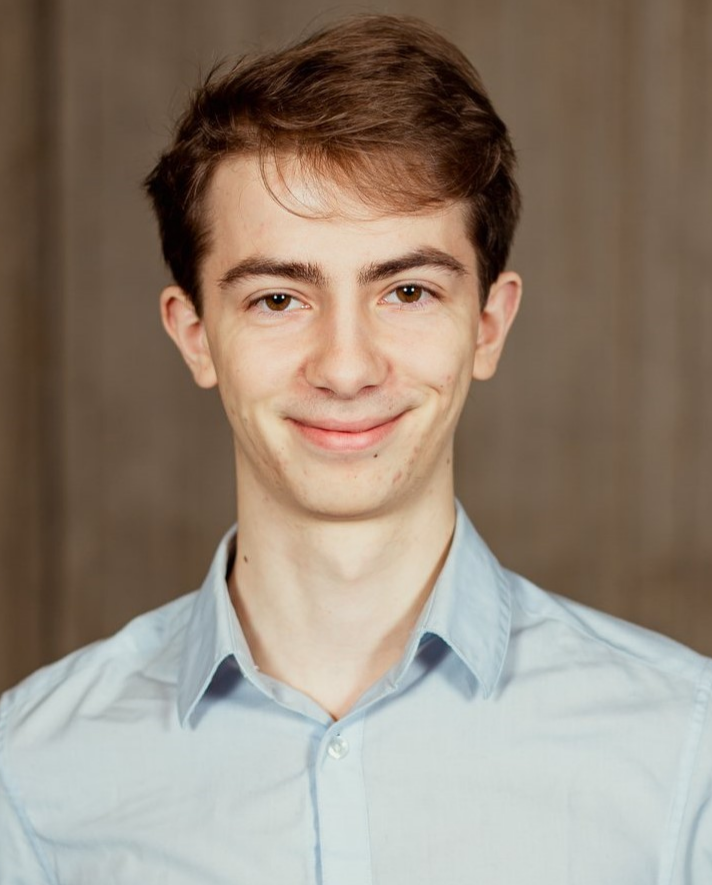
\includegraphics[width=1in,height=1.25in,clip,keepaspectratio]{figures/rw.png}}]{Robin Wydaeghe}
\DIFadd{\hspace{0.25em}}\DIFaddend received the B.Sc. and M.Sc. degrees in engineering physics from Ghent
University, Ghent, Belgium, in 2019 and 2021, respectively. He is currently
pursuing the Ph.D. degree in engineering physics with Ghent University. His
research interests include computational electromagnetics, numerical assessment
of human radiofrequency electromagnetic-field exposure, and propagation
modeling for next-generation wireless networks.
\DIFdelbegin %DIFDELCMD < \end{IEEEbiographynophoto}
%DIFDELCMD < %%%
\DIFdelend \DIFaddbegin \end{IEEEbiography}
\DIFaddend

\DIFdelbegin %DIFDELCMD < \begin{IEEEbiographynophoto}{G\"unter Vermeeren}
%DIFDELCMD < %%%
\DIFdelend \DIFaddbegin \begin{IEEEbiography}[{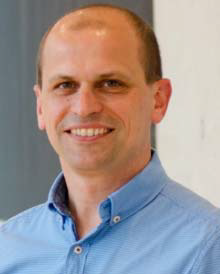
\includegraphics[width=1in,height=1.25in,clip,keepaspectratio]{figures/gv.png}}]{G\"unter Vermeeren}
\DIFadd{\hspace{0.25em}}\DIFaddend received the M.Sc. degree in industrial engineering from KAHO Sint-Lieven,
Ghent, Belgium, in 1998, the M.Sc. degree in electrical engineering from Ghent
University, Belgium, in 2001, and the Ph.D. degree in electro-technical
engineering from Ghent University in 2013. Since 2002, he has been a Research
Engineer with the Department of Information Technology, Ghent University. His
research interests include numerical modeling and measurements of
electromagnetic radiation in the domain of radiofrequency dosimetry,
electromagnetic exposure, on-body propagation, and medical imaging systems.
\DIFdelbegin %DIFDELCMD < \end{IEEEbiographynophoto}
%DIFDELCMD < %%%
\DIFdelend \DIFaddbegin \end{IEEEbiography}
\DIFaddend

\DIFdelbegin %DIFDELCMD < \begin{IEEEbiographynophoto}{Emmeric Tanghe}
%DIFDELCMD < %%%
\DIFdelend \DIFaddbegin \begin{IEEEbiography}[{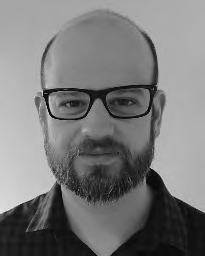
\includegraphics[width=1in,height=1.25in,clip,keepaspectratio]{figures/et.png}}]{Emmeric Tanghe}
\DIFadd{\hspace{0.25em}}\DIFaddend received the M.Sc. and Ph.D. degrees in electrical engineering from Ghent
University, Ghent, Belgium, in 2005 and 2011, respectively. In 2015, he became
a Part-Time Professor in medical applications of electromagnetic fields in and
around the human body. Since 2011, he has been a Postdoctoral Researcher with
Ghent University/IMEC, where he focuses on propagation modeling. From 2012 to
2018, he was a Postdoctoral Fellow of FWO-V (Research Foundation-Flanders).
\DIFdelbegin %DIFDELCMD < \end{IEEEbiographynophoto}
%DIFDELCMD < %%%
\DIFdelend \DIFaddbegin \end{IEEEbiography}
\DIFaddend

\DIFdelbegin %DIFDELCMD < \begin{IEEEbiographynophoto}{Wout Joseph}
%DIFDELCMD < %%%
\DIFdelend \DIFaddbegin \begin{IEEEbiography}[{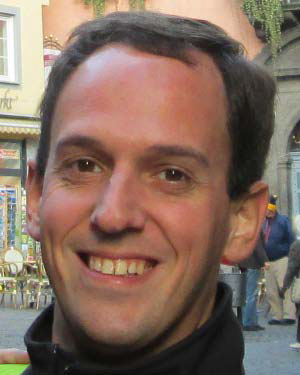
\includegraphics[width=1in,height=1.25in,clip,keepaspectratio]{figures/wj.png}}]{Wout Joseph}
\DIFadd{\hspace{0.25em}}\DIFaddend received the M.Sc. degree in electrical engineering from Ghent University,
Ghent, Belgium, in 2000, and the Ph.D. degree in electrical engineering from
Ghent University in 2005. Since 2009, he has been a Professor in the domain of
experimental characterization of wireless communication systems. His research
interests include measuring and modeling electromagnetic fields around base
stations for mobile communications, electromagnetic exposure assessment,
propagation for wireless communication systems, and antennas and calibration.
\DIFdelbegin %DIFDELCMD < \end{IEEEbiographynophoto}
%DIFDELCMD <

%DIFDELCMD < \EOD
%DIFDELCMD < %%%
\DIFdelend \DIFaddbegin \end{IEEEbiography}
\DIFaddend

\end{document}
